\documentclass[fleqn]{article}
\oddsidemargin 0.0in
\textwidth 6.0in
\thispagestyle{empty}
\usepackage{import}
\usepackage{amsmath}
\usepackage{graphicx}
\usepackage{flexisym}
\usepackage{calligra}
\usepackage{amssymb}
\usepackage{bigints} 
\usepackage[english]{babel}
\usepackage[utf8x]{inputenc}
\usepackage{float}
\usepackage[colorinlistoftodos]{todonotes}


\DeclareMathAlphabet{\mathcalligra}{T1}{calligra}{m}{n}
\DeclareFontShape{T1}{calligra}{m}{n}{<->s*[2.2]callig15}{}
\newcommand{\scriptr}{\mathcalligra{r}\,}
\newcommand{\boldscriptr}{\pmb{\mathcalligra{r}}\,}

\definecolor{hwColor}{HTML}{AD53BA}

\begin{document}

  \begin{titlepage}

    \newcommand{\HRule}{\rule{\linewidth}{0.5mm}}

    \center

    \begin{center}
      
\includegraphics[height=11cm, width=11cm]{asu.png}
    \end{center}

    \vline

    \textsc{\LARGE Classical Parts/Field/Matter II}\\[1.5cm]

    \HRule \\[0.5cm]
    { \huge \bfseries Problem Set Five}\\[0.4cm] 
    \HRule \\[1.0cm]

    \textbf{Behnam Amiri}

    \bigbreak

    \textbf{Prof: Maulik Parikh}

    \bigbreak

    \textbf{{\large \today}\\[2cm]}

    \vfill

  \end{titlepage}

  \begin{enumerate}
    \item The magnetic field at the surface of a neutron star can reach a value of $10^{10}$ (!) Teslas. Suppose that it takes that value 
    (and points vertically up) at the magnetic north pole of the star, and assume that the magnetic field is roughly that of a dipole. 
    Imagine that the source of the field were modeled as a current ring on the equator of the neutron star (radius 10 $km$). How large 
    would the current have to be?

    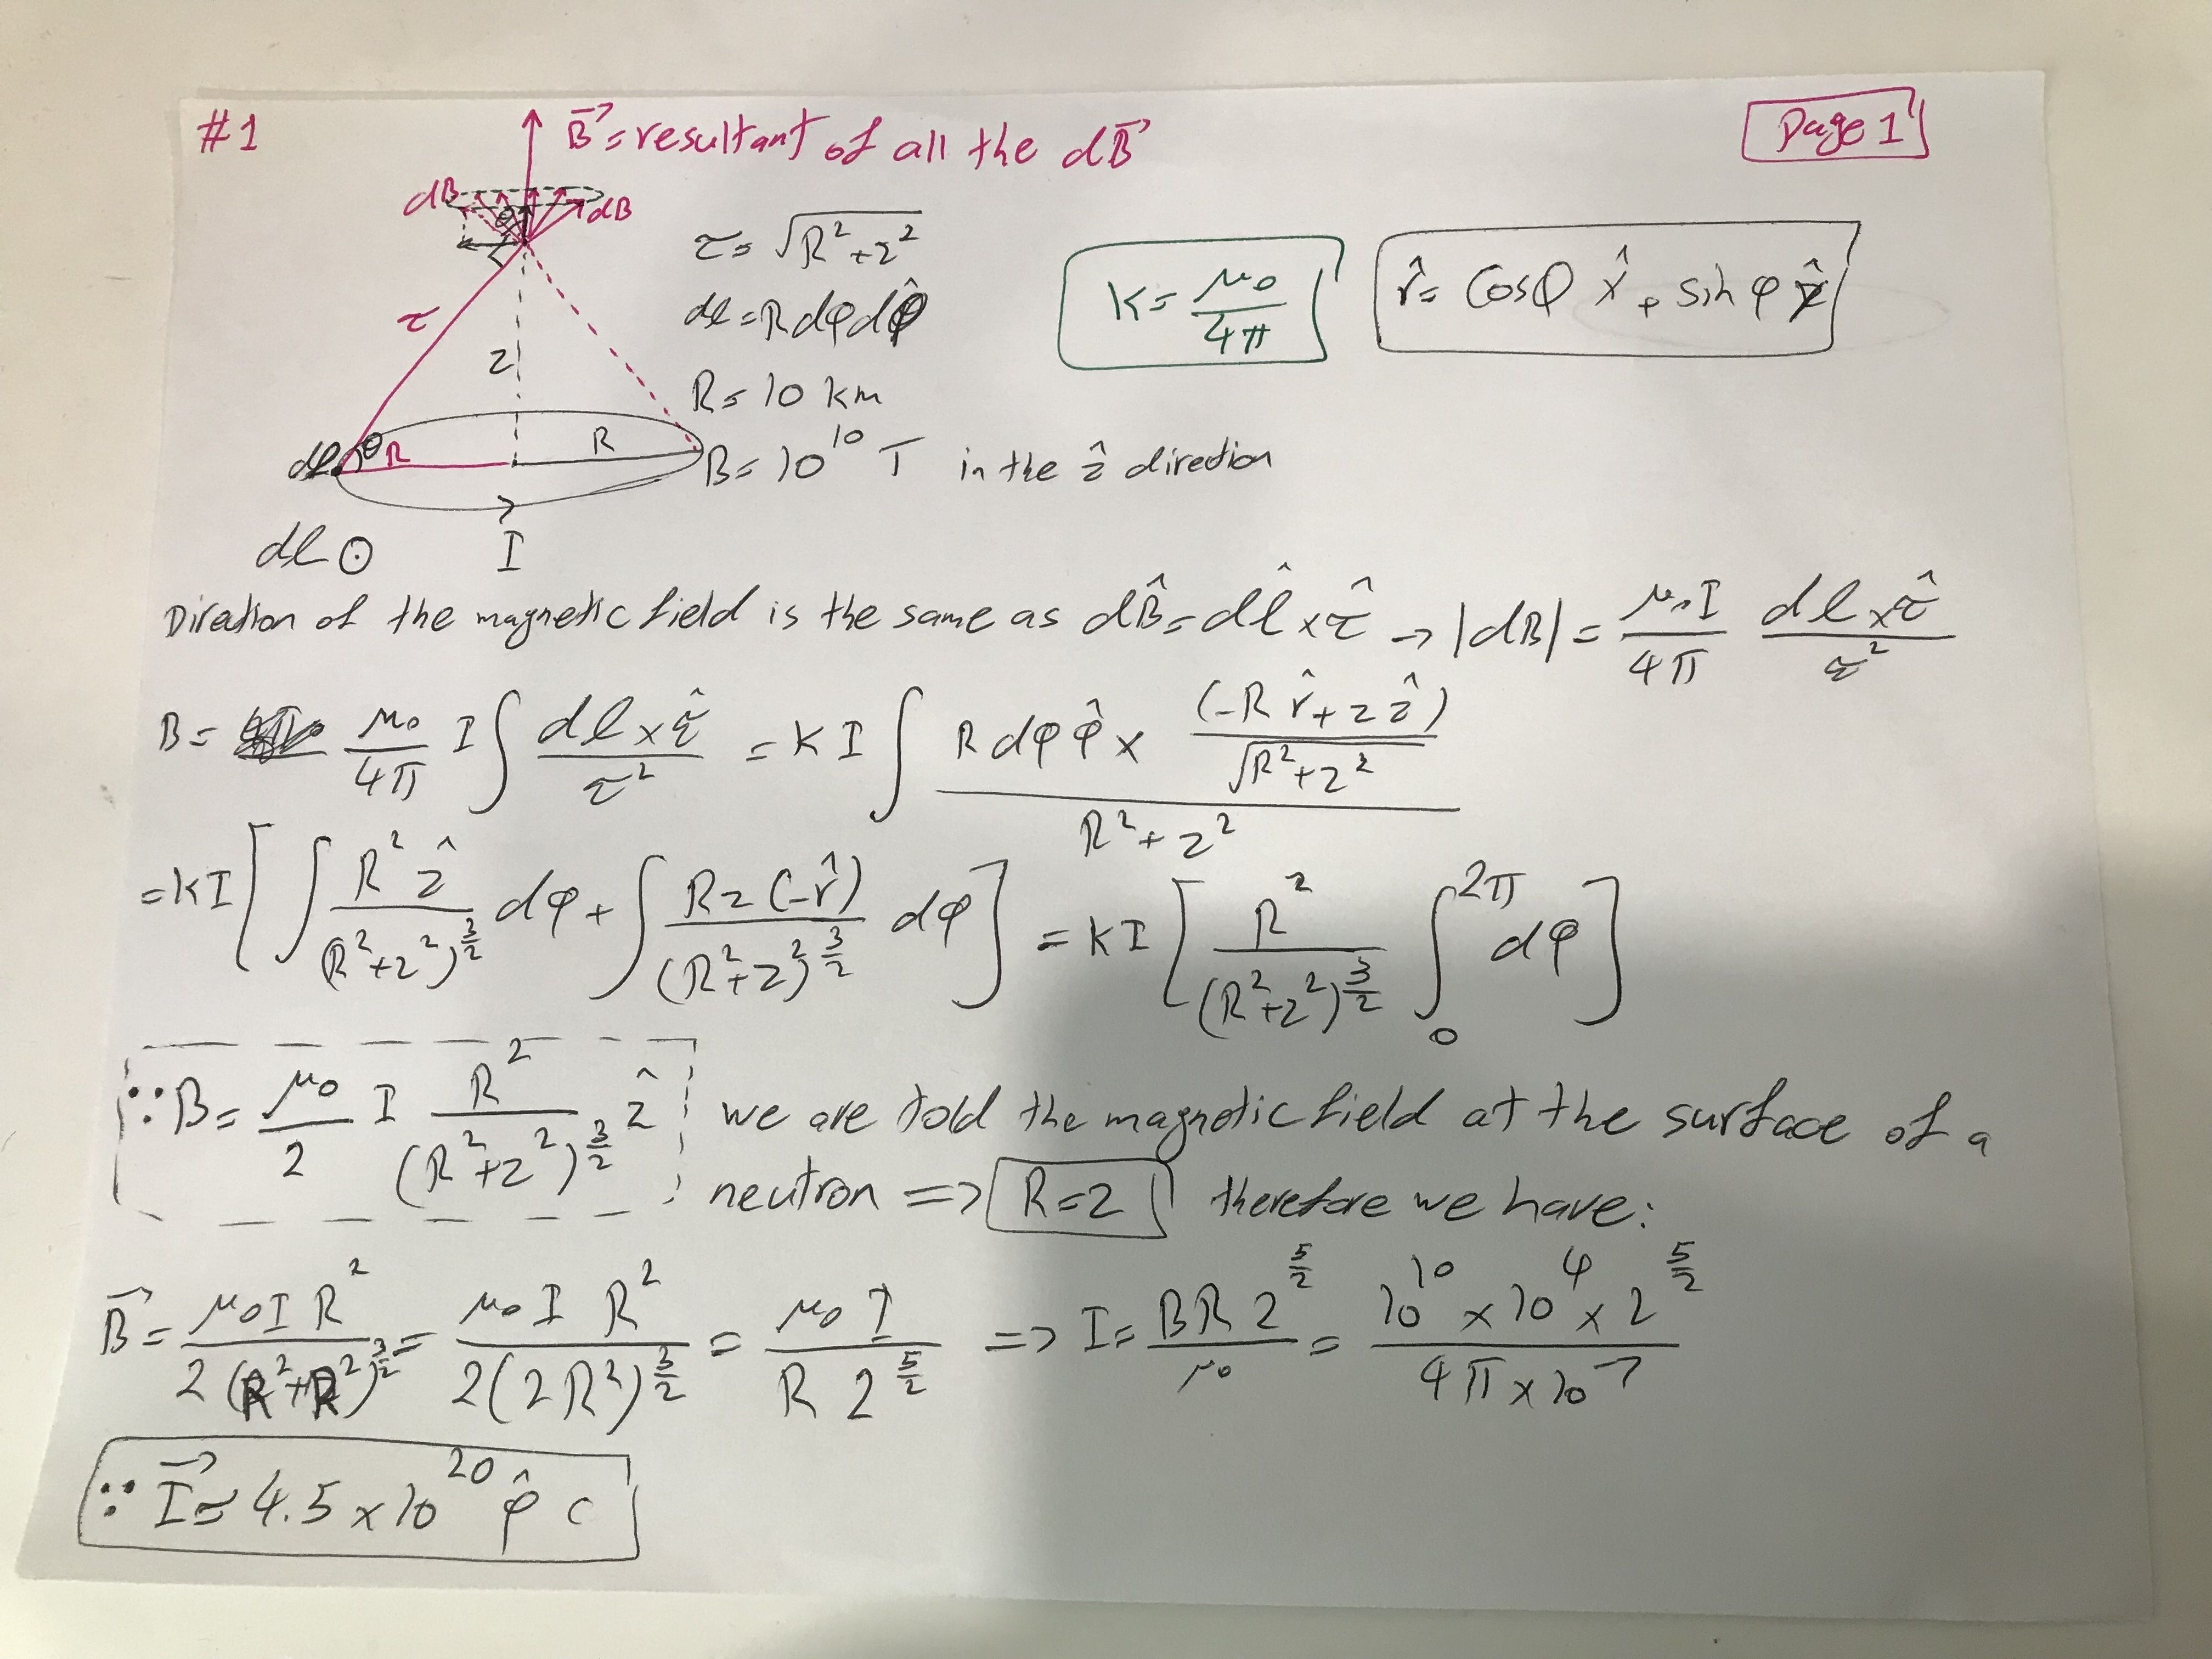
\includegraphics[height=13cm, width=15cm]{1.jpg}

    \pagebreak

    \item Consider a time-dependent charge density:
    $$
      \rho(t, \overrightarrow{r})=\rho_0 \dfrac{e^{-bt}}{r}
    $$
    where $b$ and $\rho_0$ are dimensionful constants. Find the current density $\overrightarrow{J}(t, \overrightarrow{r})$.

    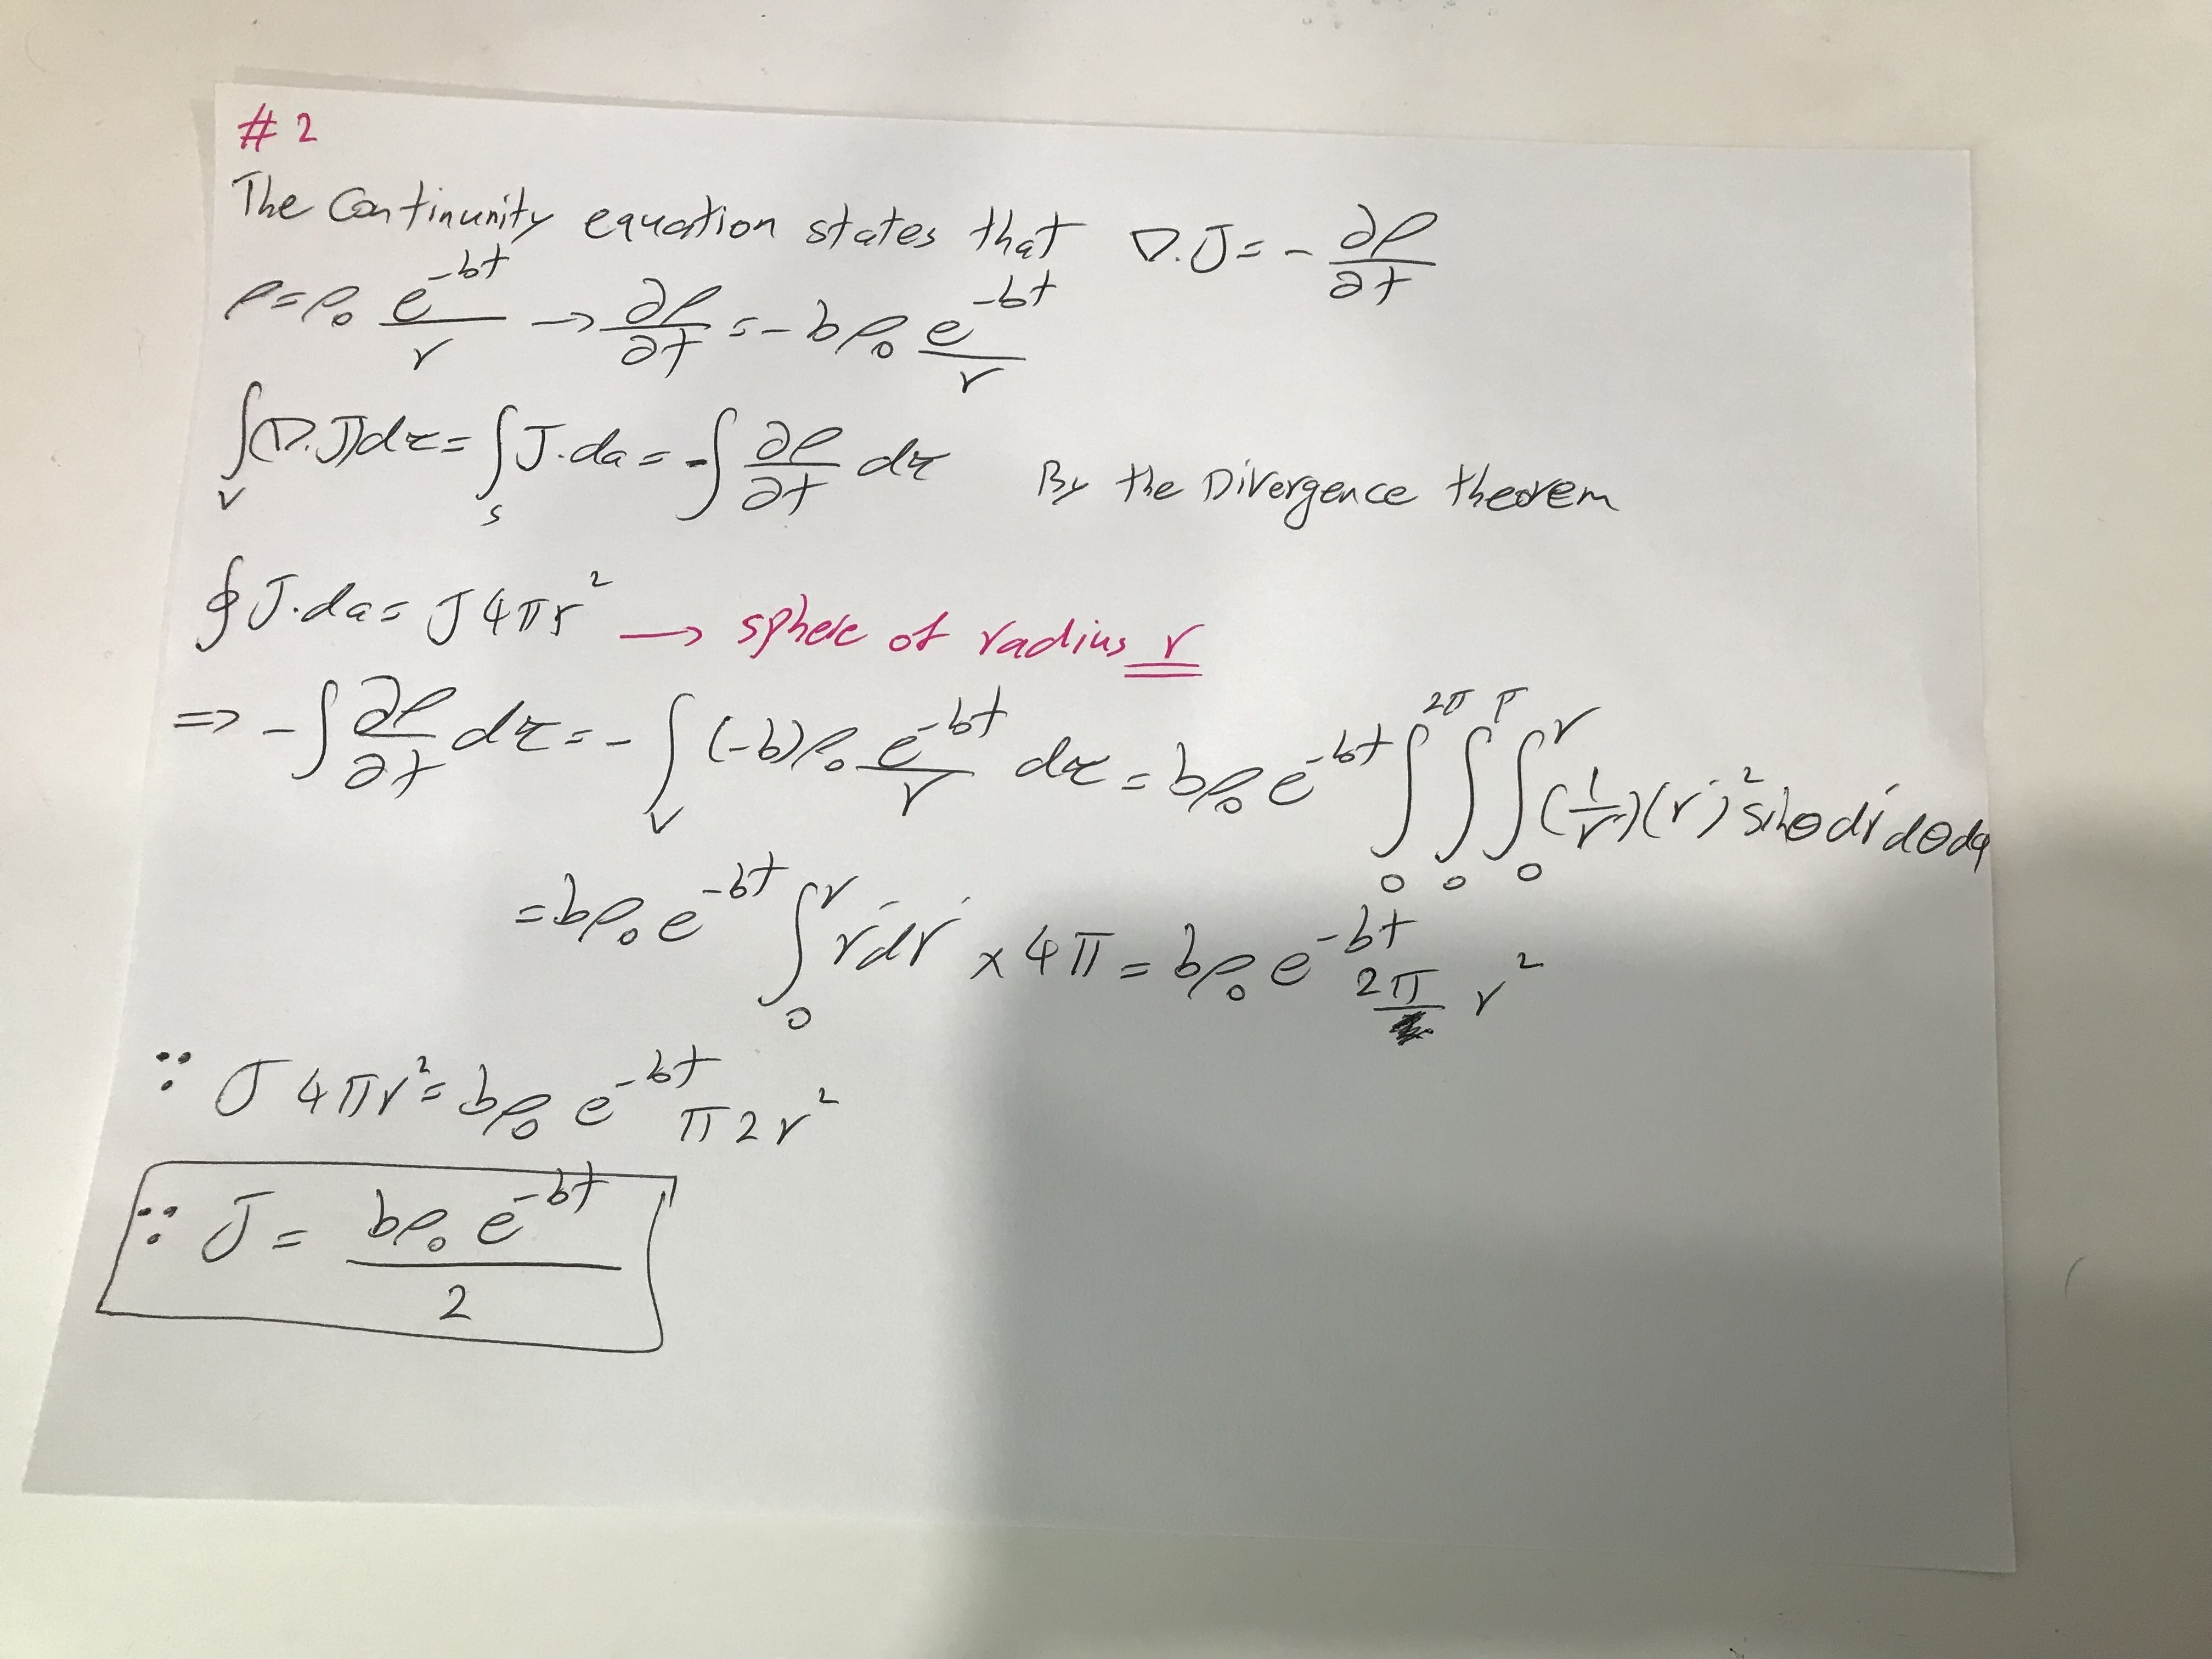
\includegraphics[height=13cm, width=15cm]{2.jpg}

    \pagebreak

    \item The Lagrangian for a particle with mass $m$ and charge $q$ and velocity 
    $\overrightarrow{v}=\dot{\overrightarrow{r}}$ in an electromagnetic field is
    $$
      L\left(
        \overrightarrow{r}(t), \dot{\overrightarrow{r}}(t)
      \right)=\dfrac{1}{2} m \overrightarrow{v}^2-qV(x,y,z)+q \overrightarrow{A}(x,y,z).\overrightarrow{v}
    $$
    Calculate the equation of motion for each Cartesian component of $\overrightarrow{r}(t)$. Write the three 
    component equations as one vectorial equation for the force, $\overrightarrow{F}=m \ddot{\overrightarrow{r}}$. 
    What is this equation? (Recall: the Euler-Lagrange equations for $L\left(x(t), \dot{x}(t)\right)$ are 
    $\dfrac{d}{dt} \dfrac{\partial L}{\partial \dot{x}}=\dfrac{\partial L}{\partial x}$.)

    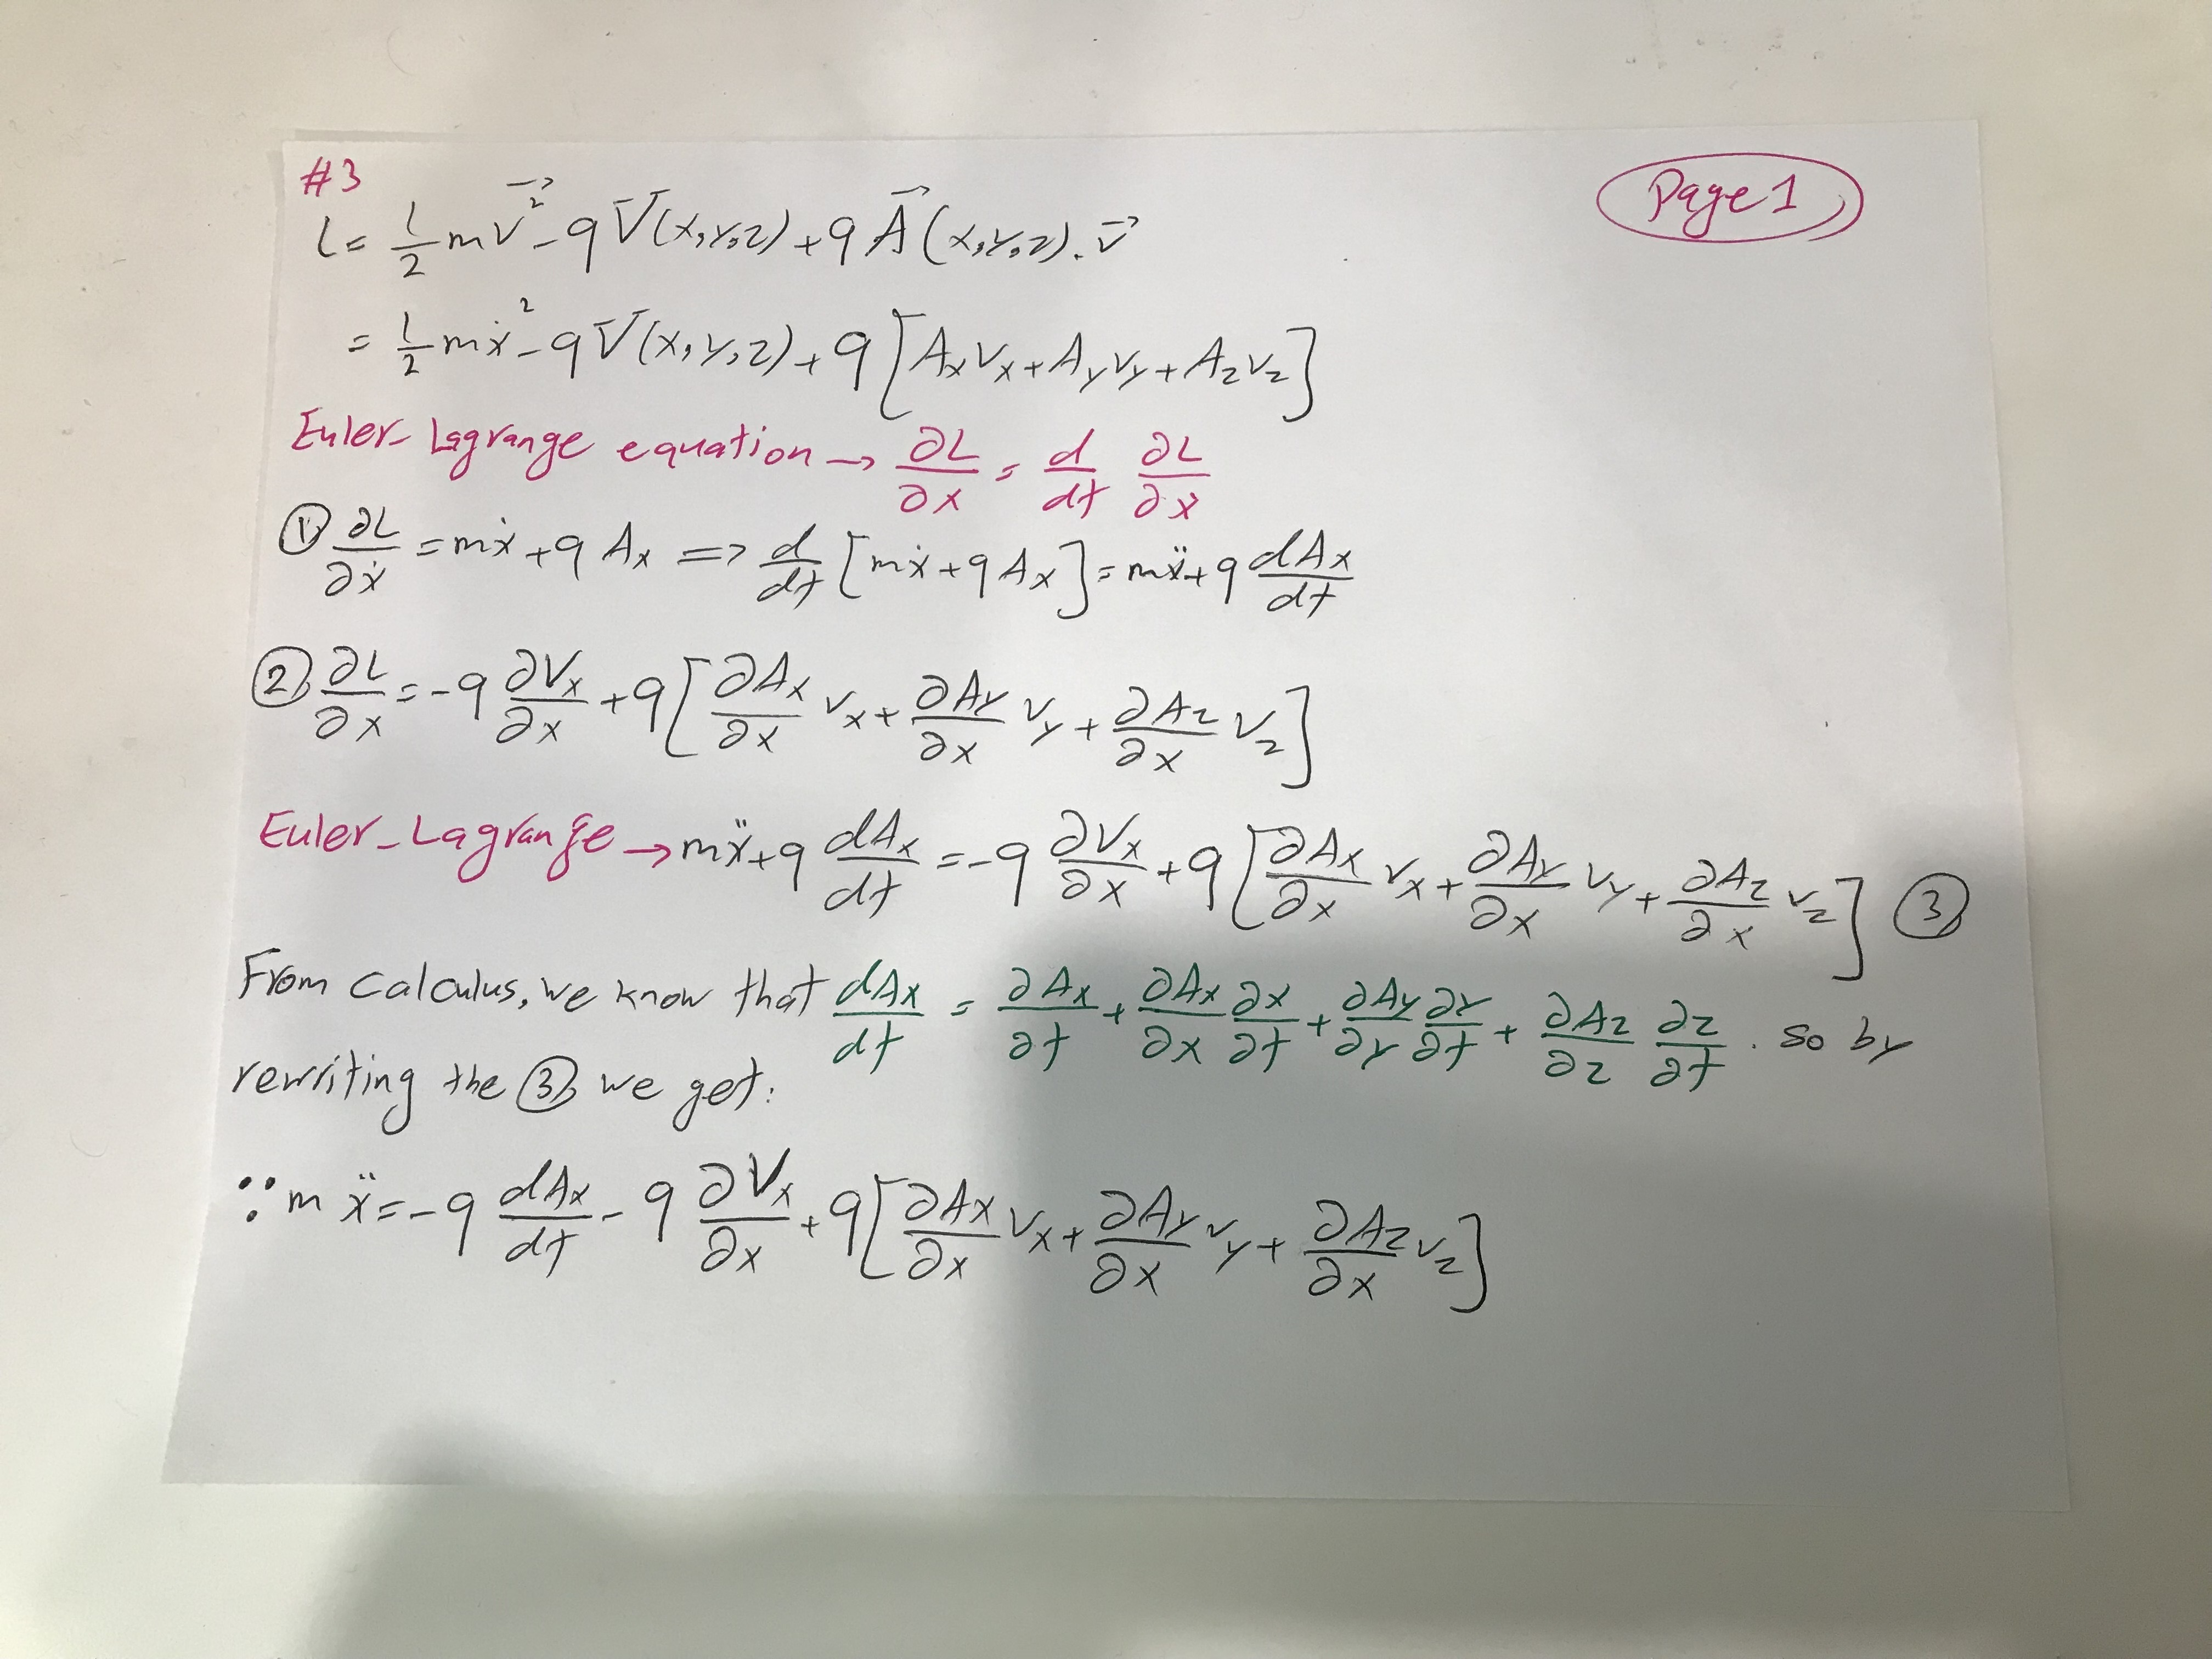
\includegraphics[height=13cm, width=15cm]{3A.jpg}

    \pagebreak

    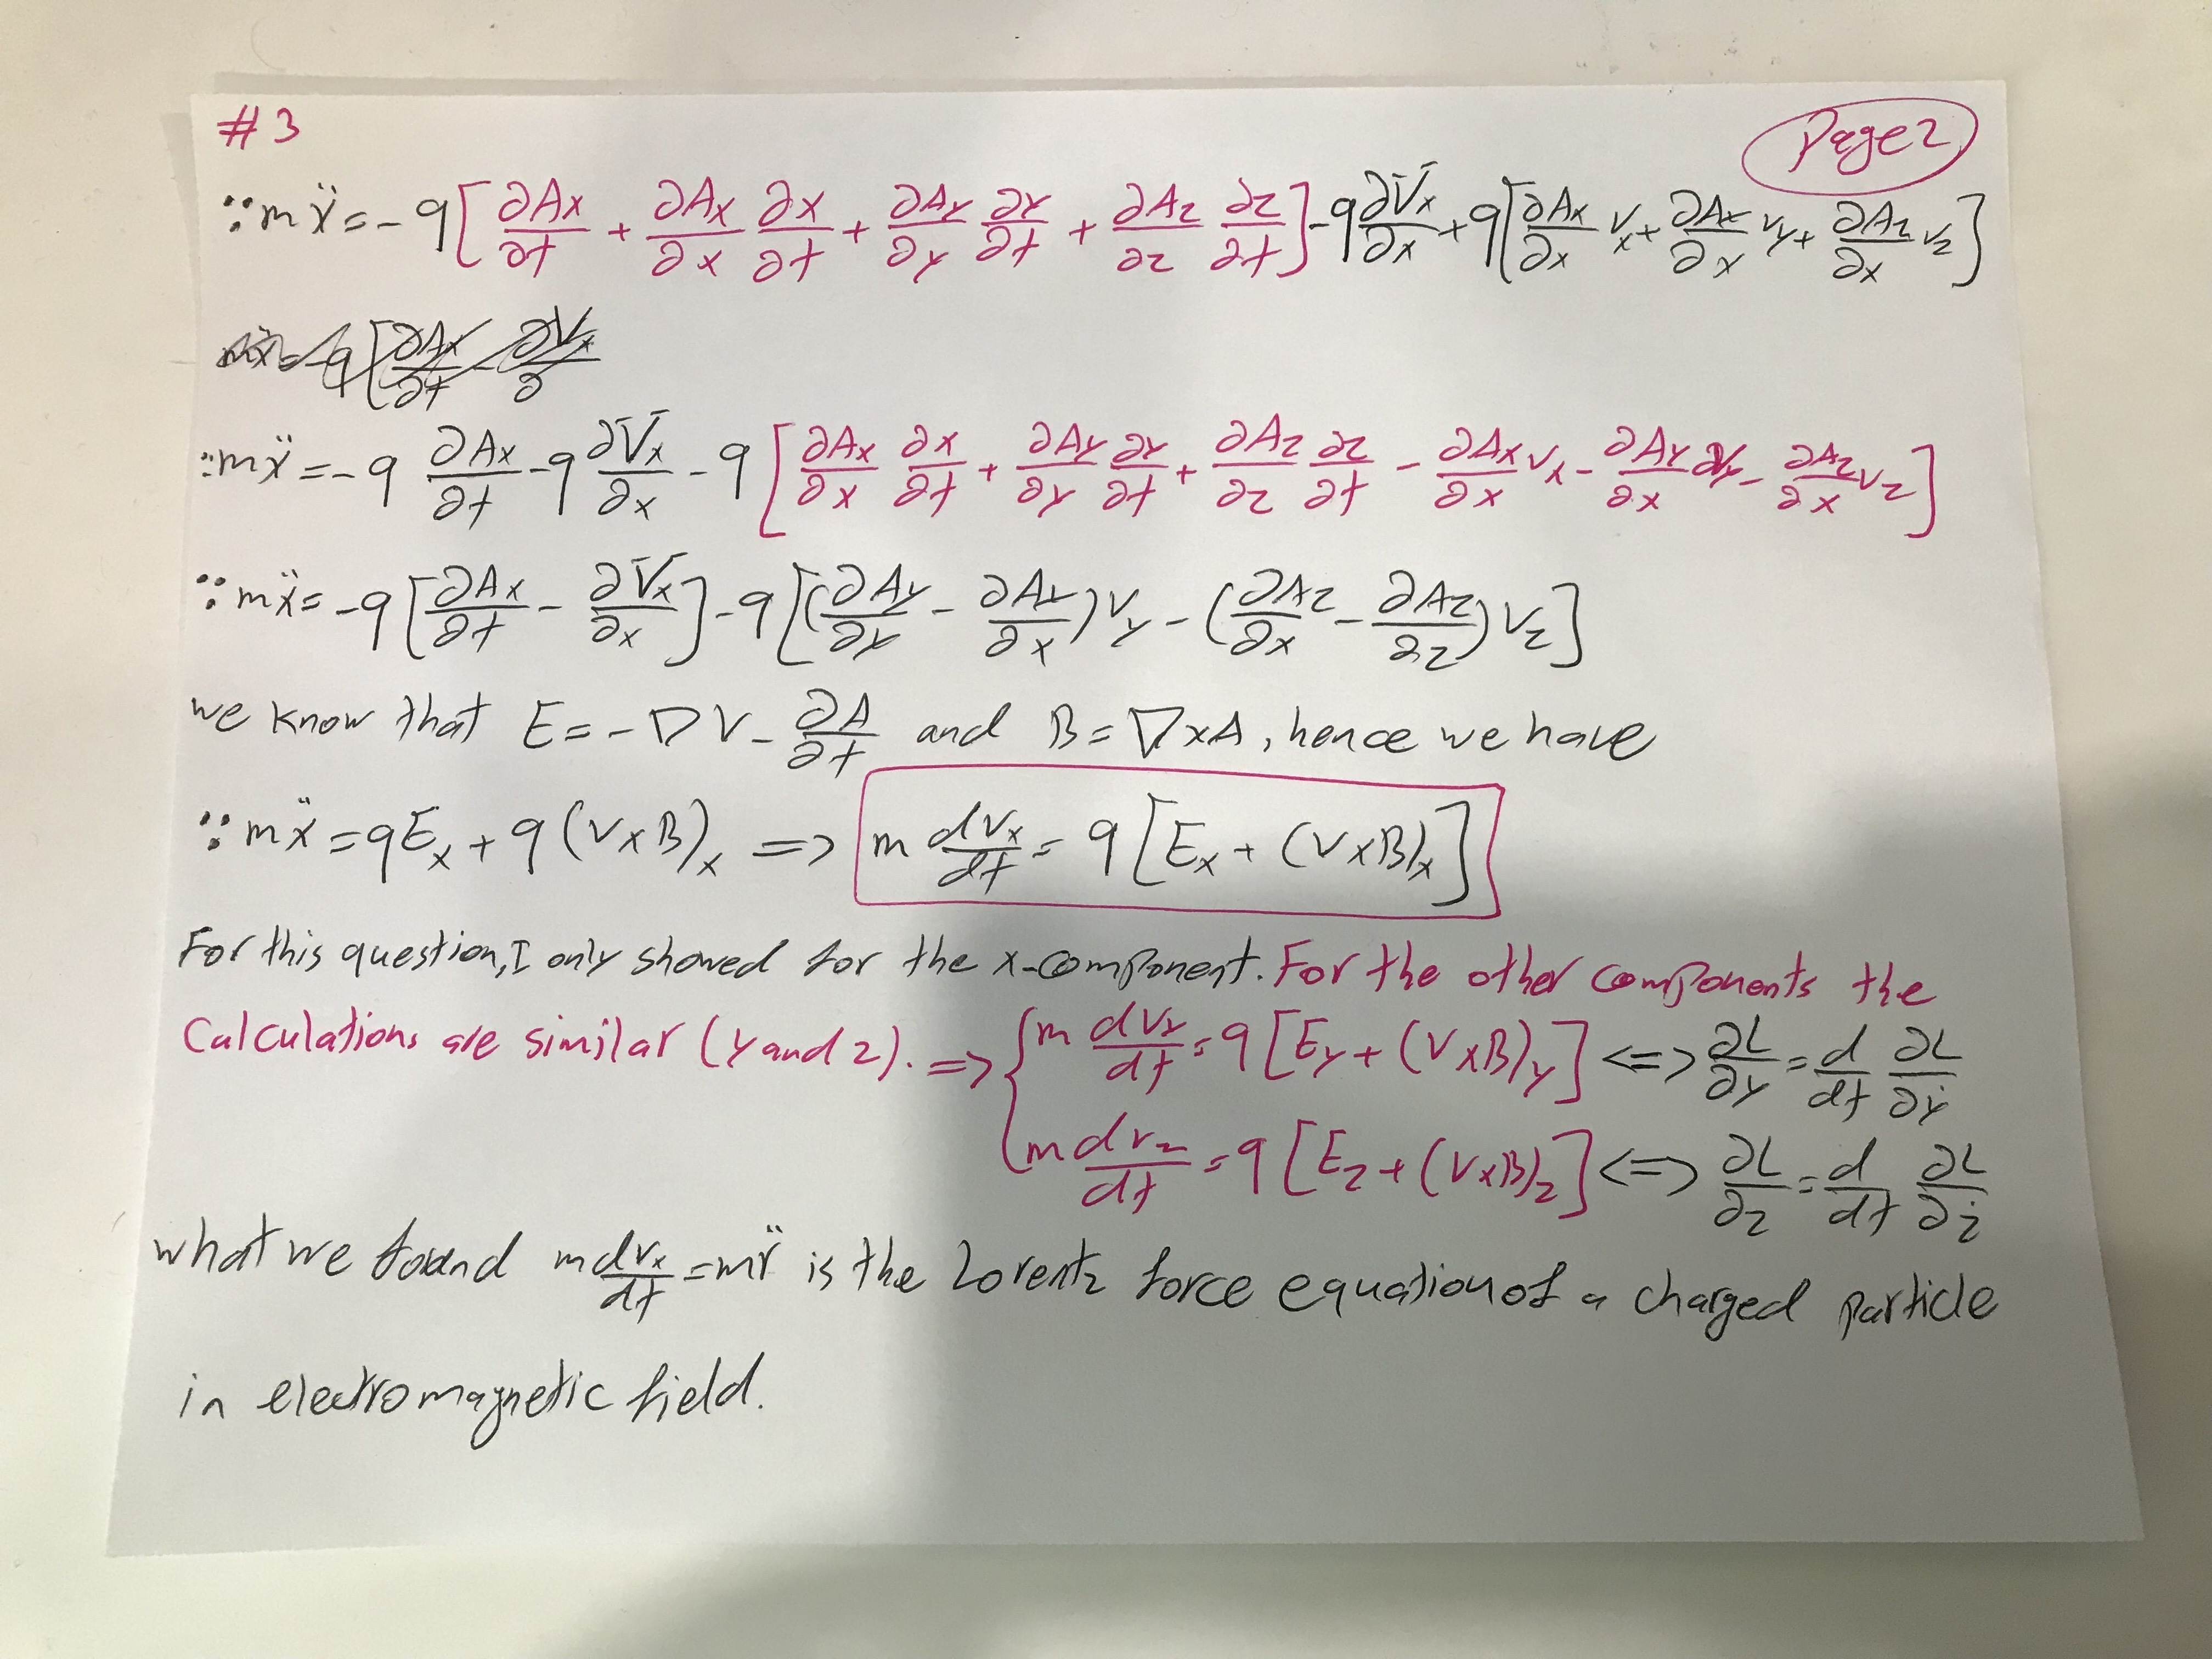
\includegraphics[height=13cm, width=15cm]{3B.jpg}

    \pagebreak

    \item An lternating current, $V(t)=V_0 sin(\omega t)$, supplies power to a light bulb of resistance $R$. 
    If a capacitor, $C$, is attached in series with the light bulb, what is the r.m.s. (root mean square) 
    brightness of the bulb as a fraction of its original r.m.s. brightness? You may assume that
    the brightness is proportional to the power dissipated in the resistor.

    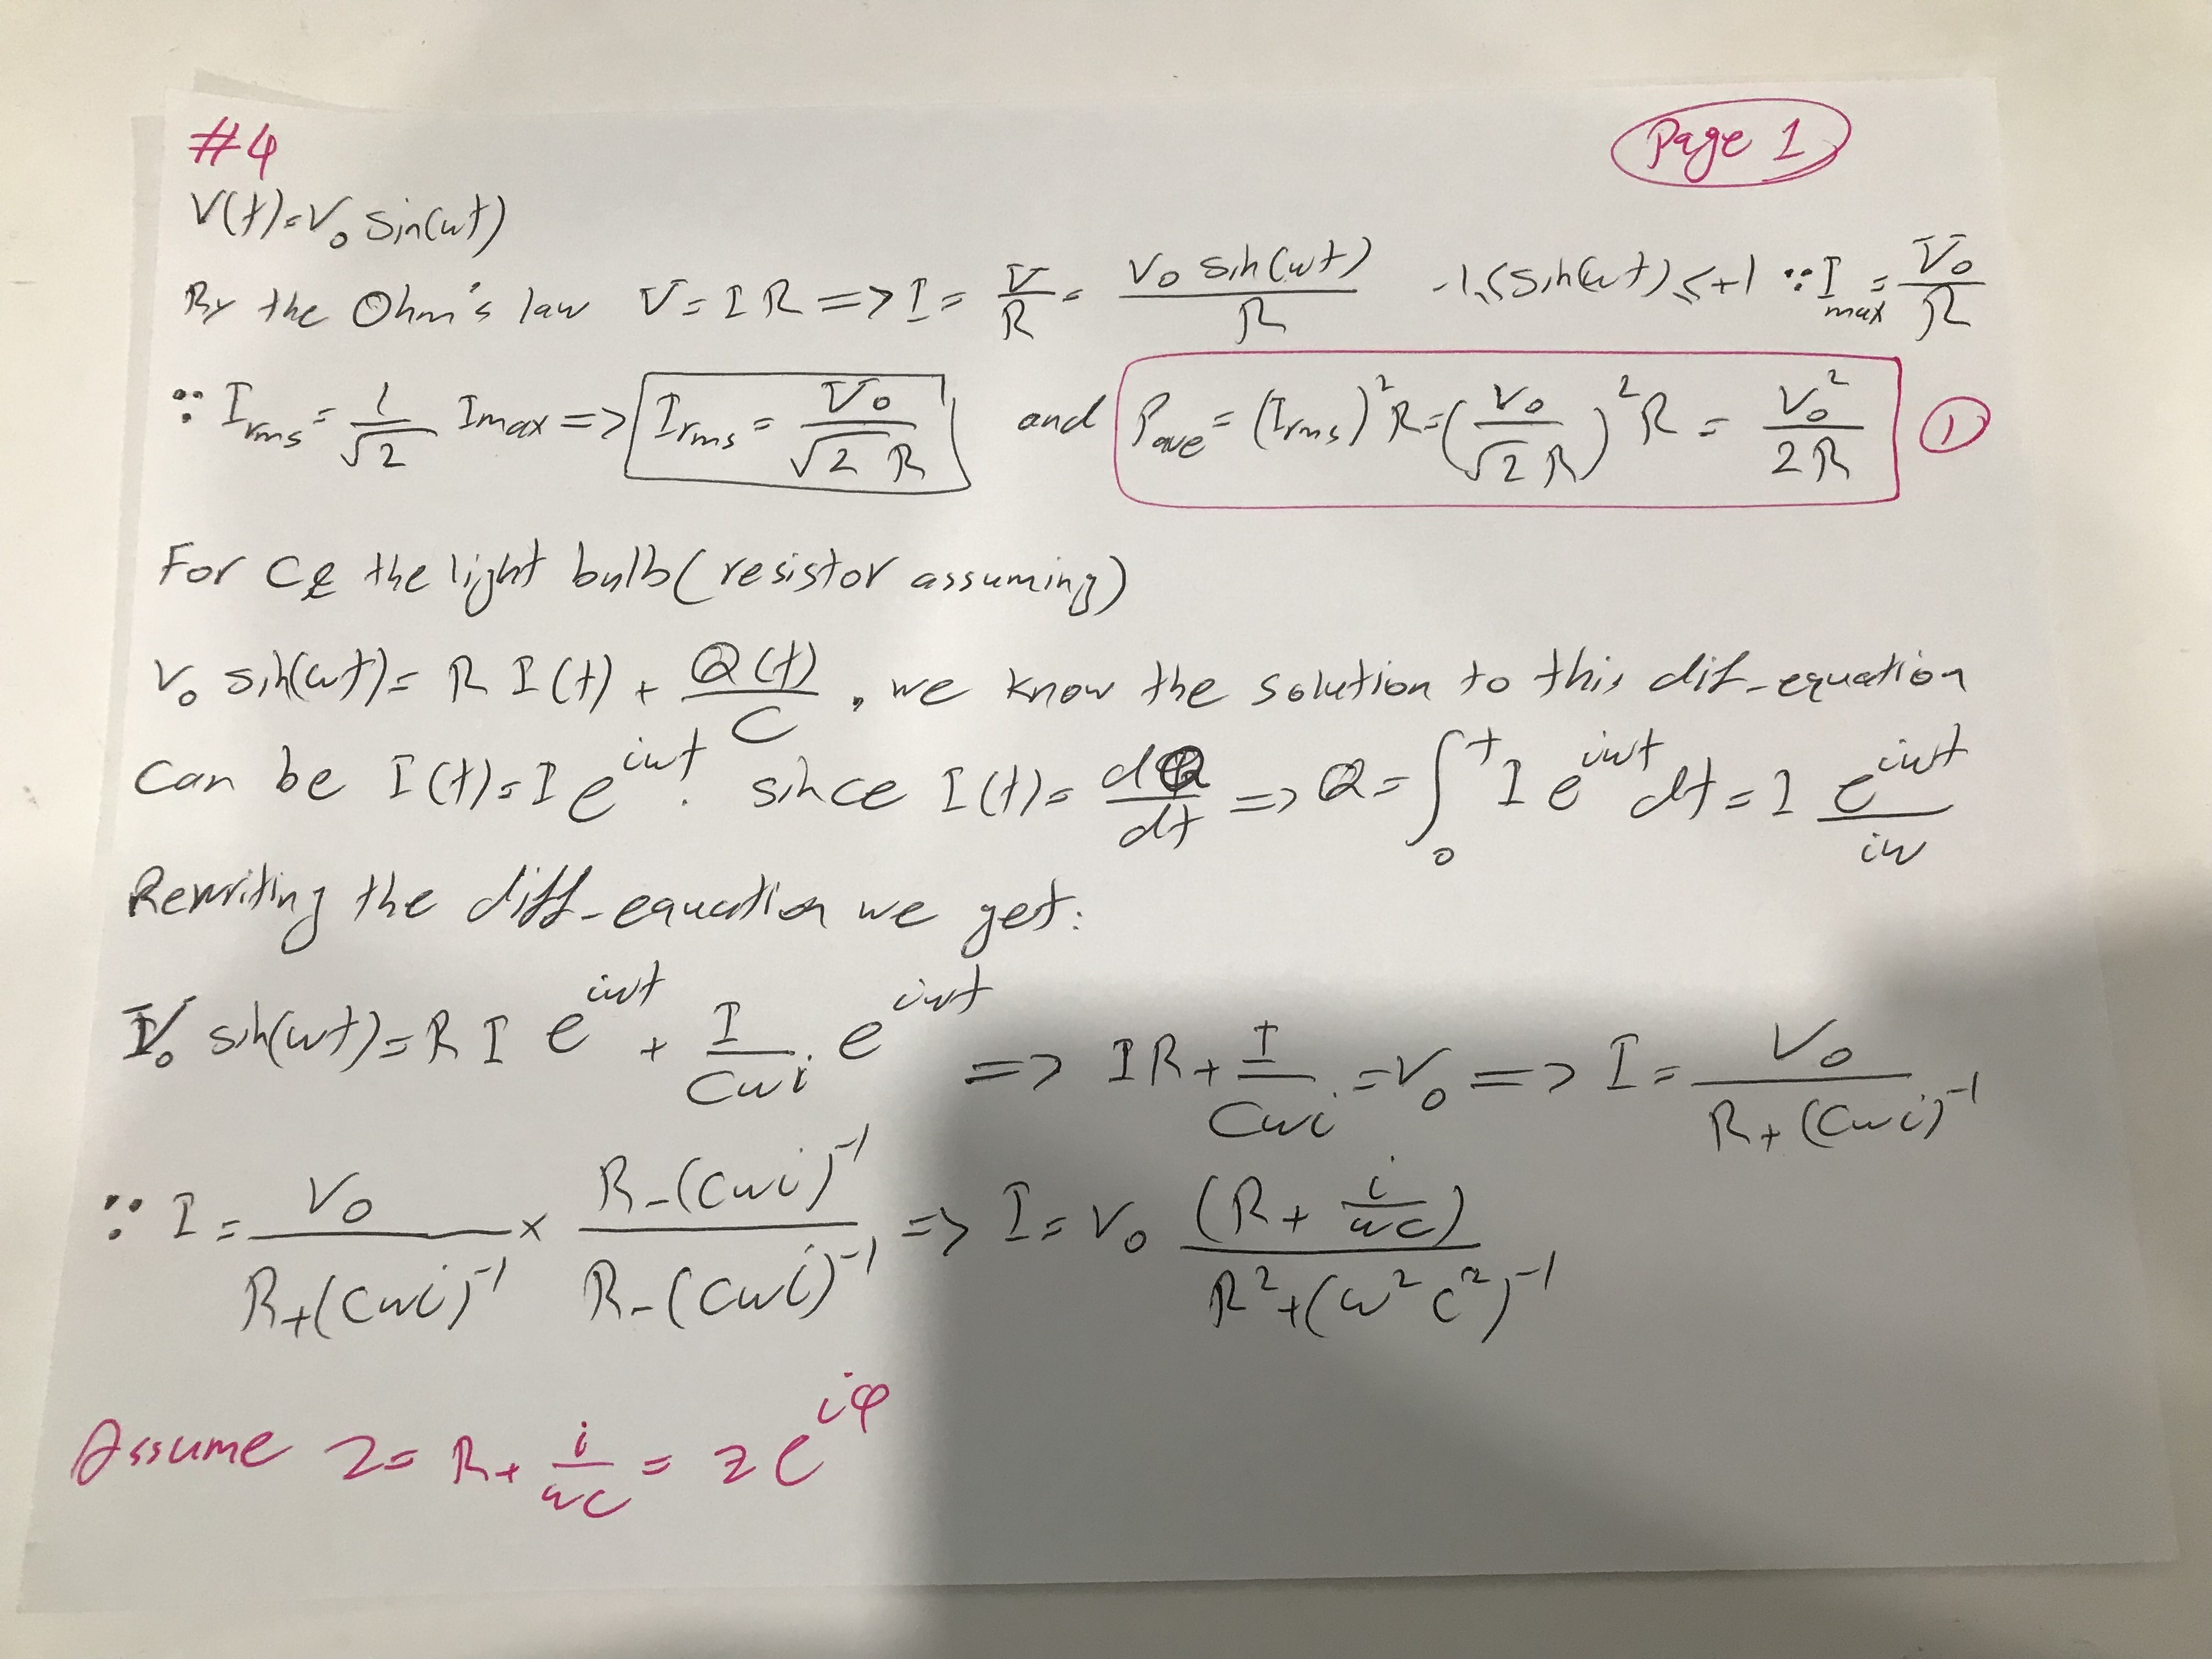
\includegraphics[height=13cm, width=15cm]{4A.jpg}

    \pagebreak

    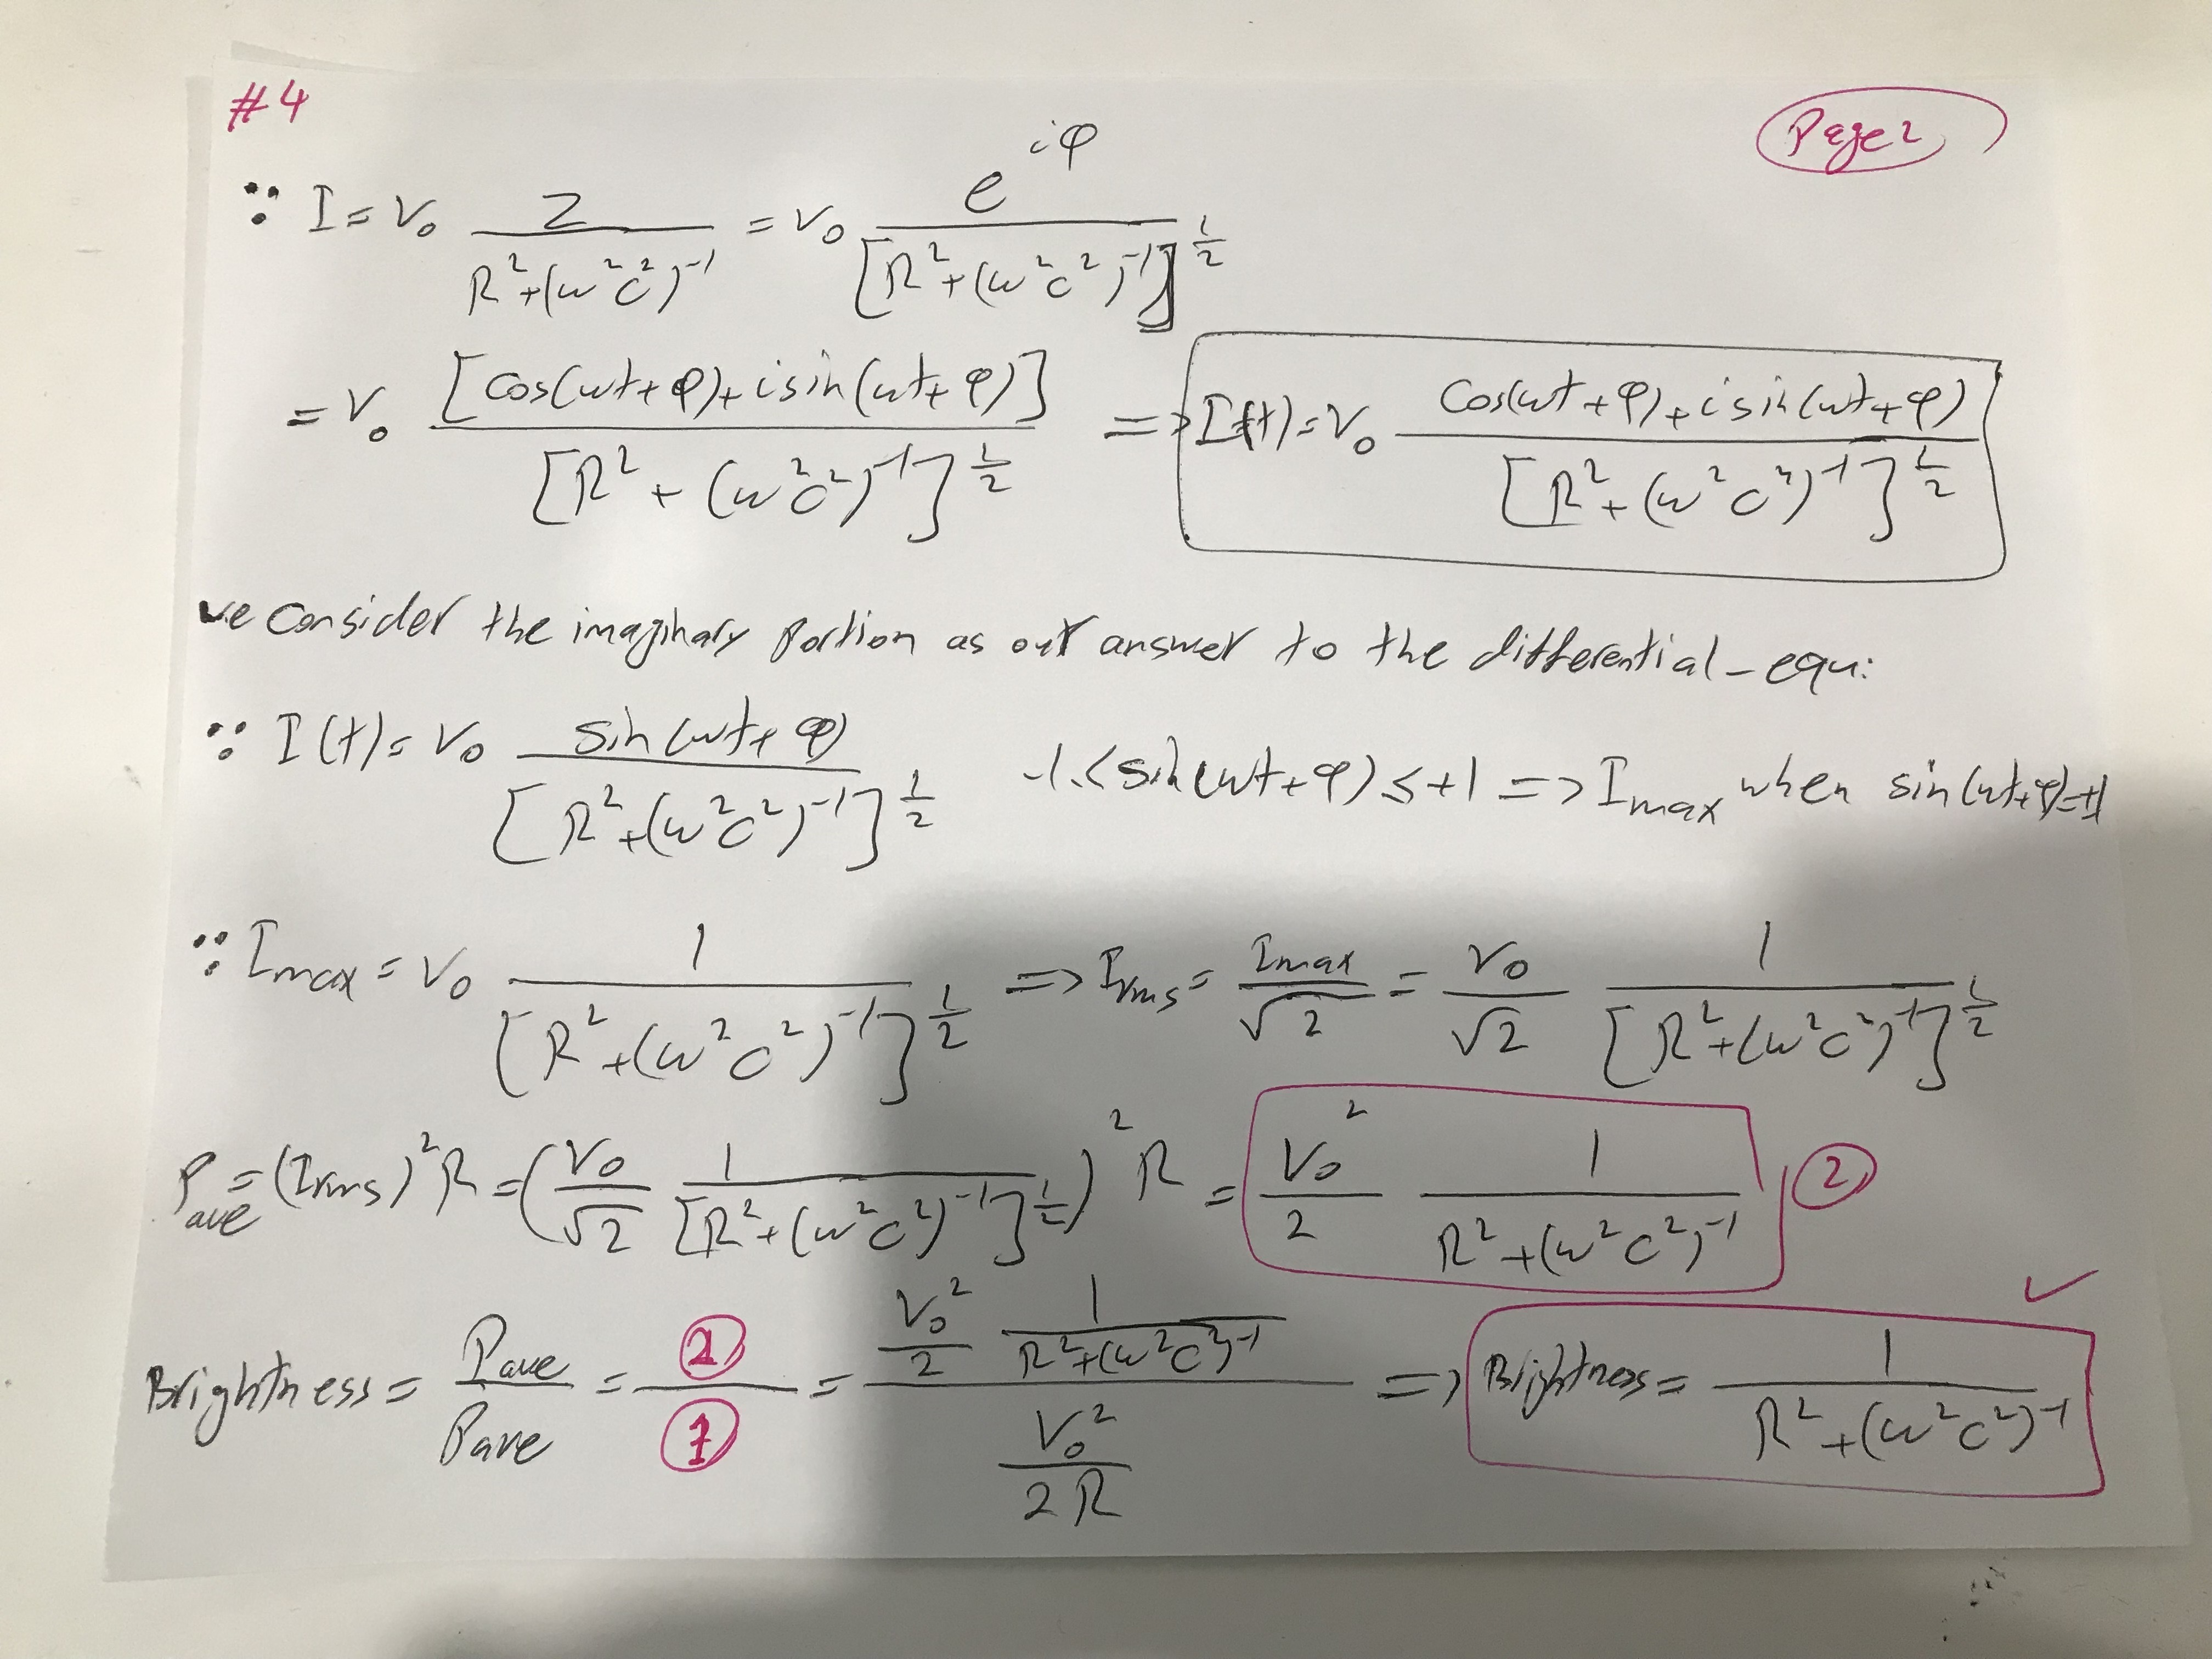
\includegraphics[height=13cm, width=15cm]{4B.jpg}

    \pagebreak

    \item A very long solenoid of radius a and height h has N closely wound turns of coil. Suppose there is a 
    slowly increasing current $I(t)$ that runs through the coils. Consider a point $P$ inside the solenoid 
    (i.e at $r < a$).
    \begin{enumerate}
      \item Find the magnetic field at $P$ (disregard the effect of the changing
      electric field on the magnetic field).

      \item Find the electric field at $P$.
    \end{enumerate}

    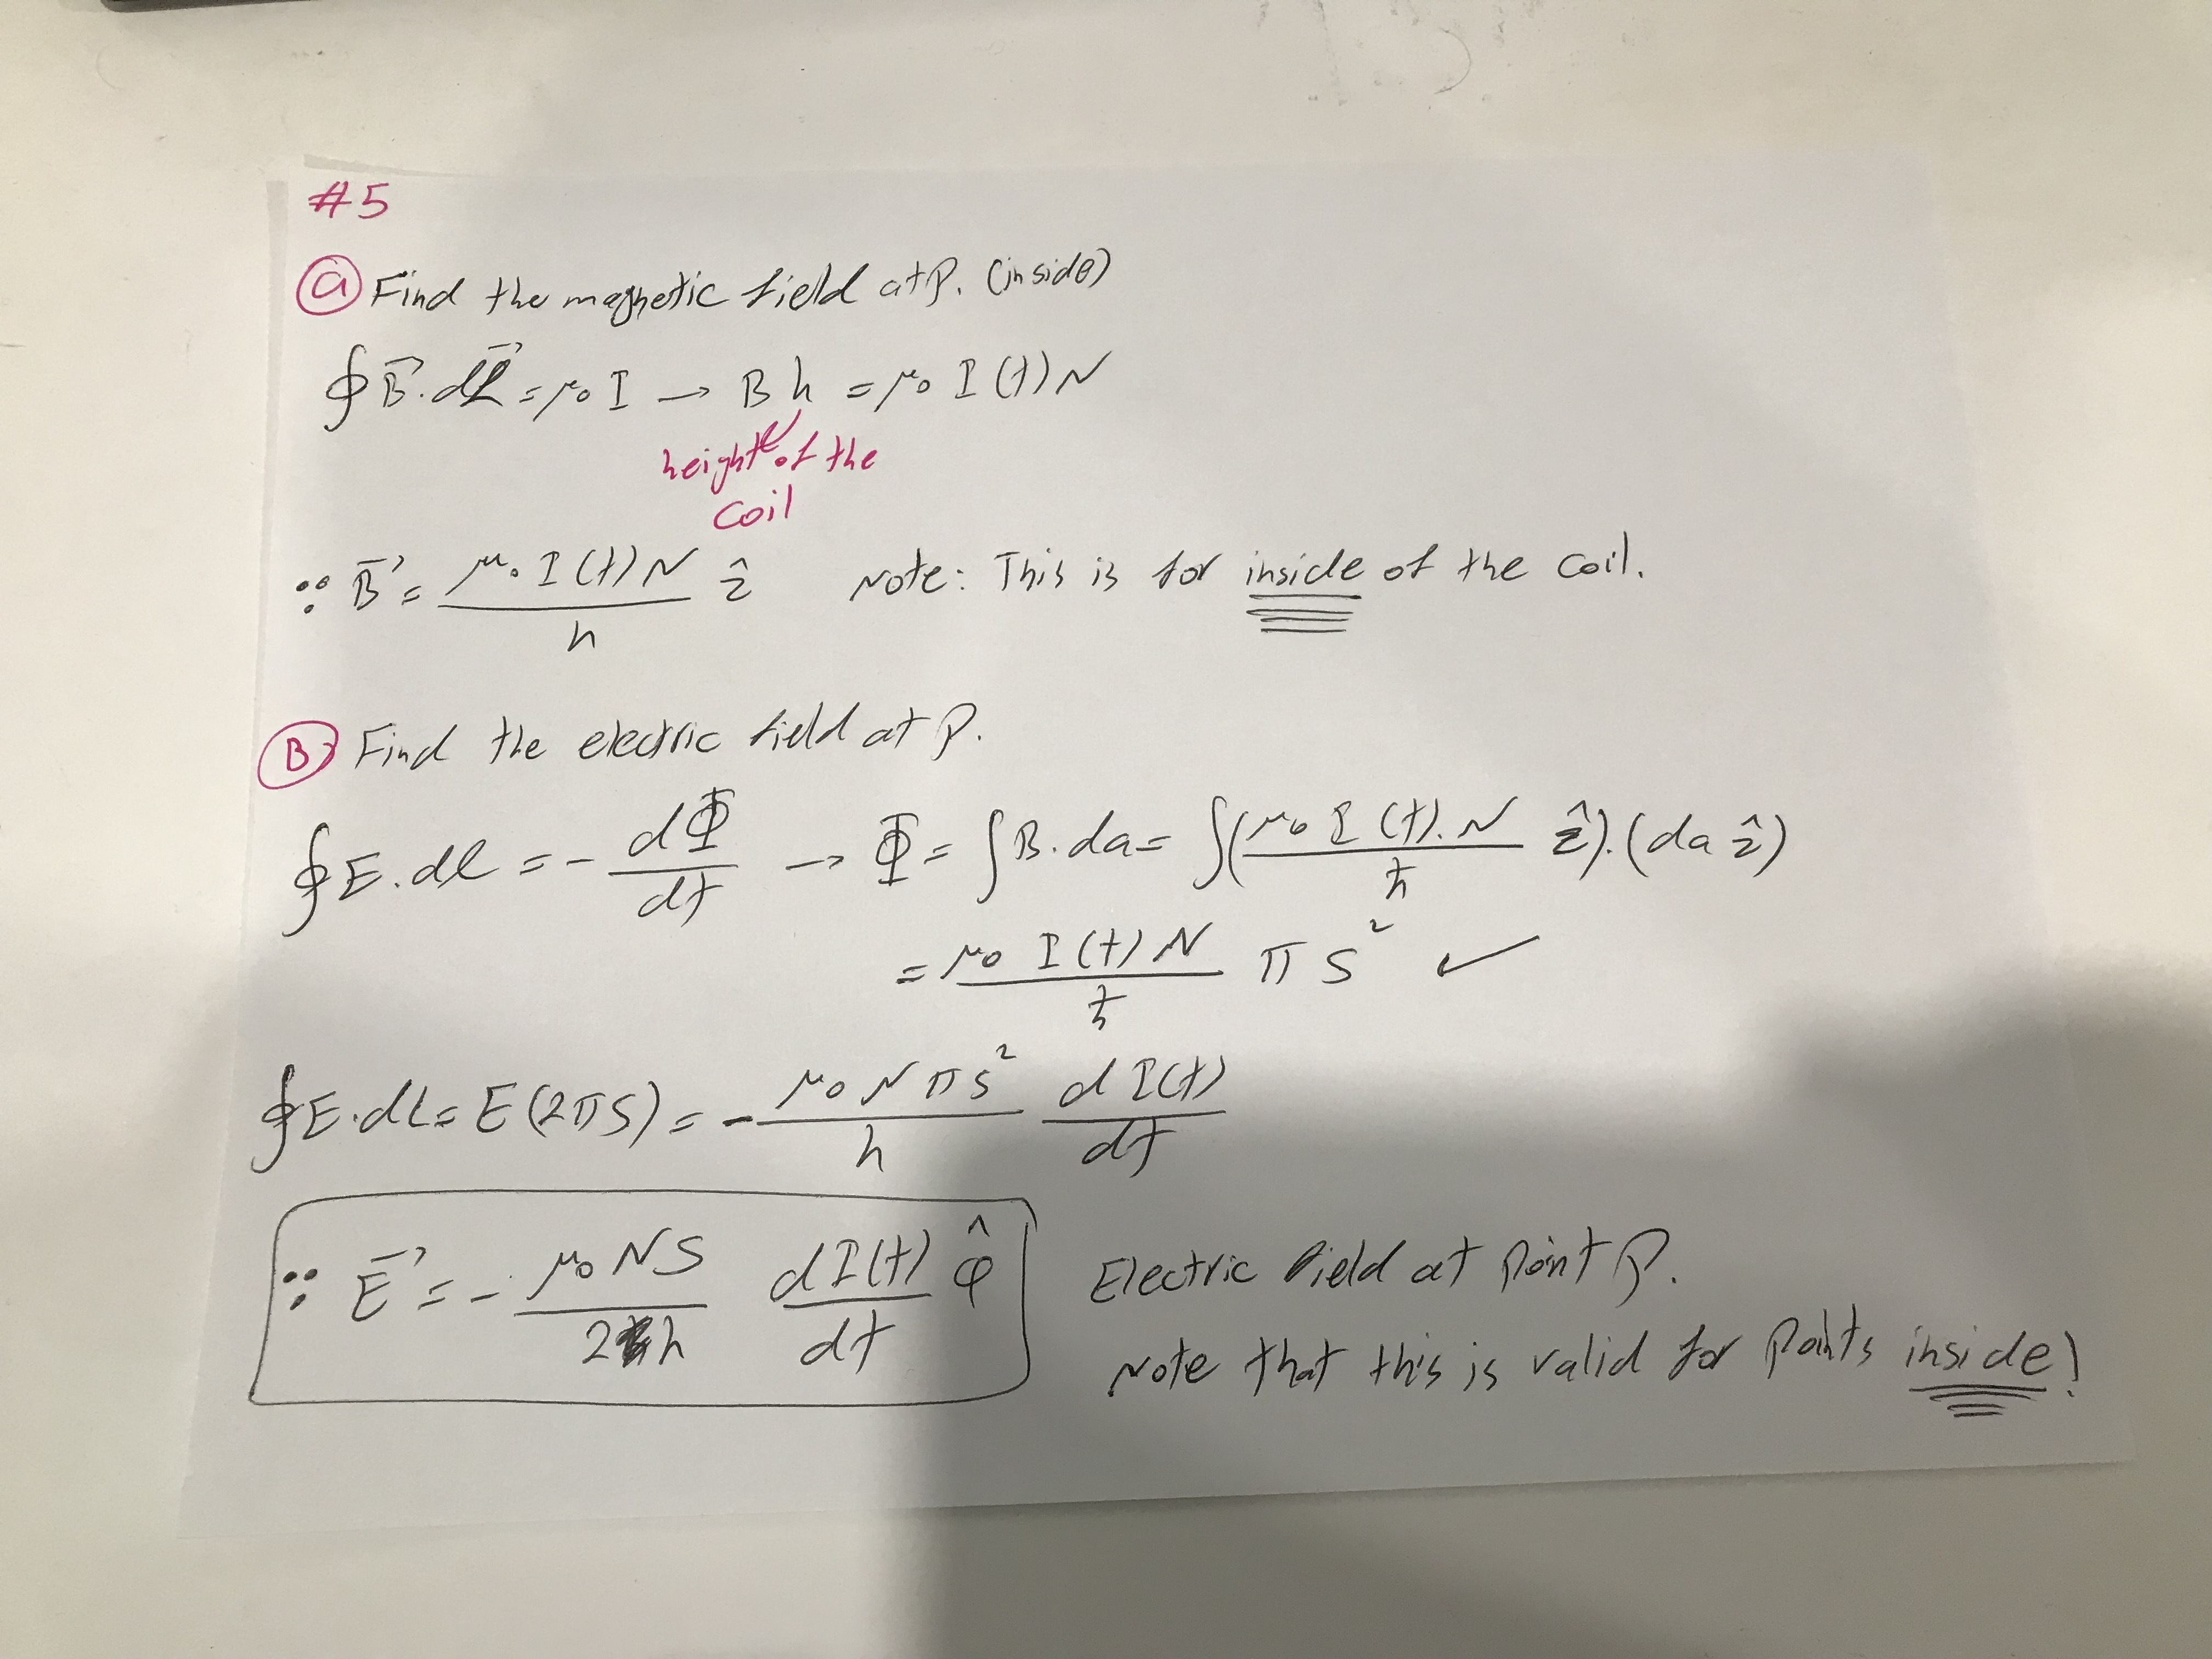
\includegraphics[height=13cm, width=15cm]{5.jpg}

    \pagebreak


    \item A wire frame shaped like a square with sides of length a has total resistance $R$. The square is oriented 
    so that two of the diagonally opposite corners lie on the x-axis. Suppose now that there is a uniform
    magnetic field $\overrightarrow{B}$ pointing out of the page throughout the region $x < 0$. The square is being 
    pulled with speed $v$ to the right i.e. out of the region where there is a magnetic field. Consider the moment 
    when the left corner is at $x_0$ where $-\dfrac{a}{\sqrt{2}} \leq x_0 <0$.
    \begin{enumerate}
      \item What force must be applied to the square so that it moves with
      constant speed $v$?

      \item how that the work done in moving the left corner from $x=x_0$ to $x=0$ (at which 
      point the square is outside the magnetized region) equals the energy dissipated in the 
      resistor.
    \end{enumerate}

    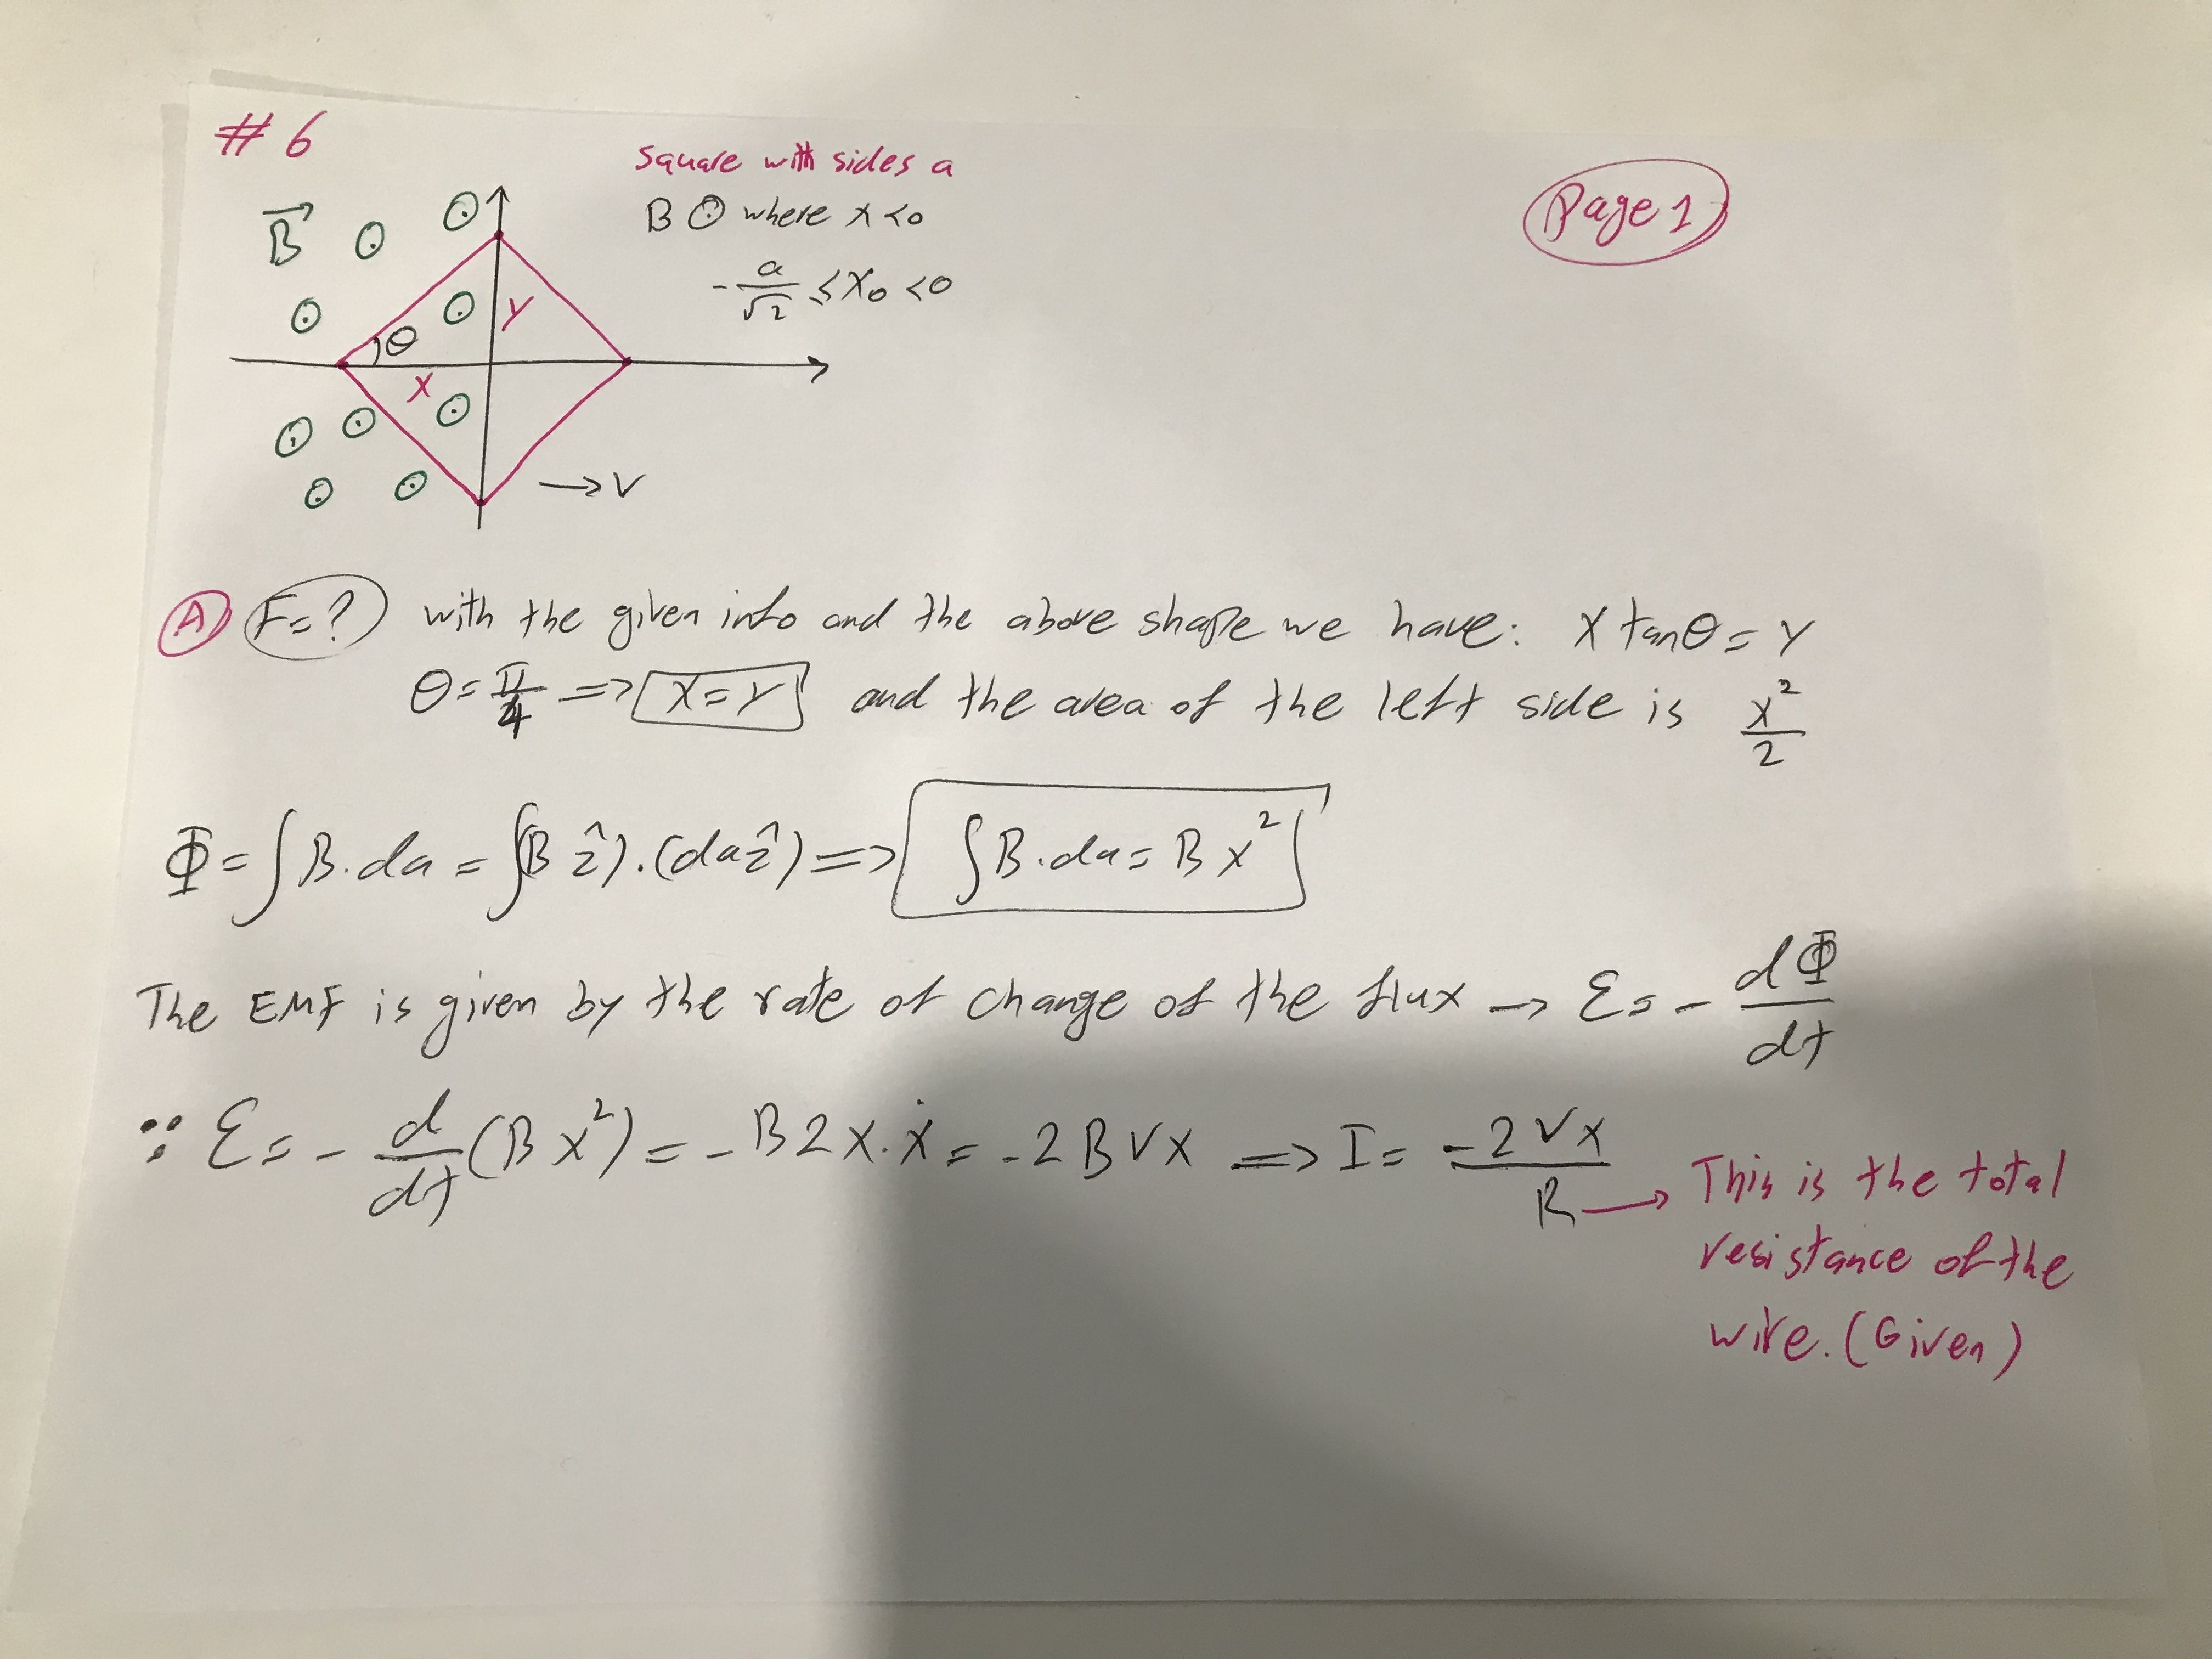
\includegraphics[height=13cm, width=15cm]{6A.jpg}

    \pagebreak

    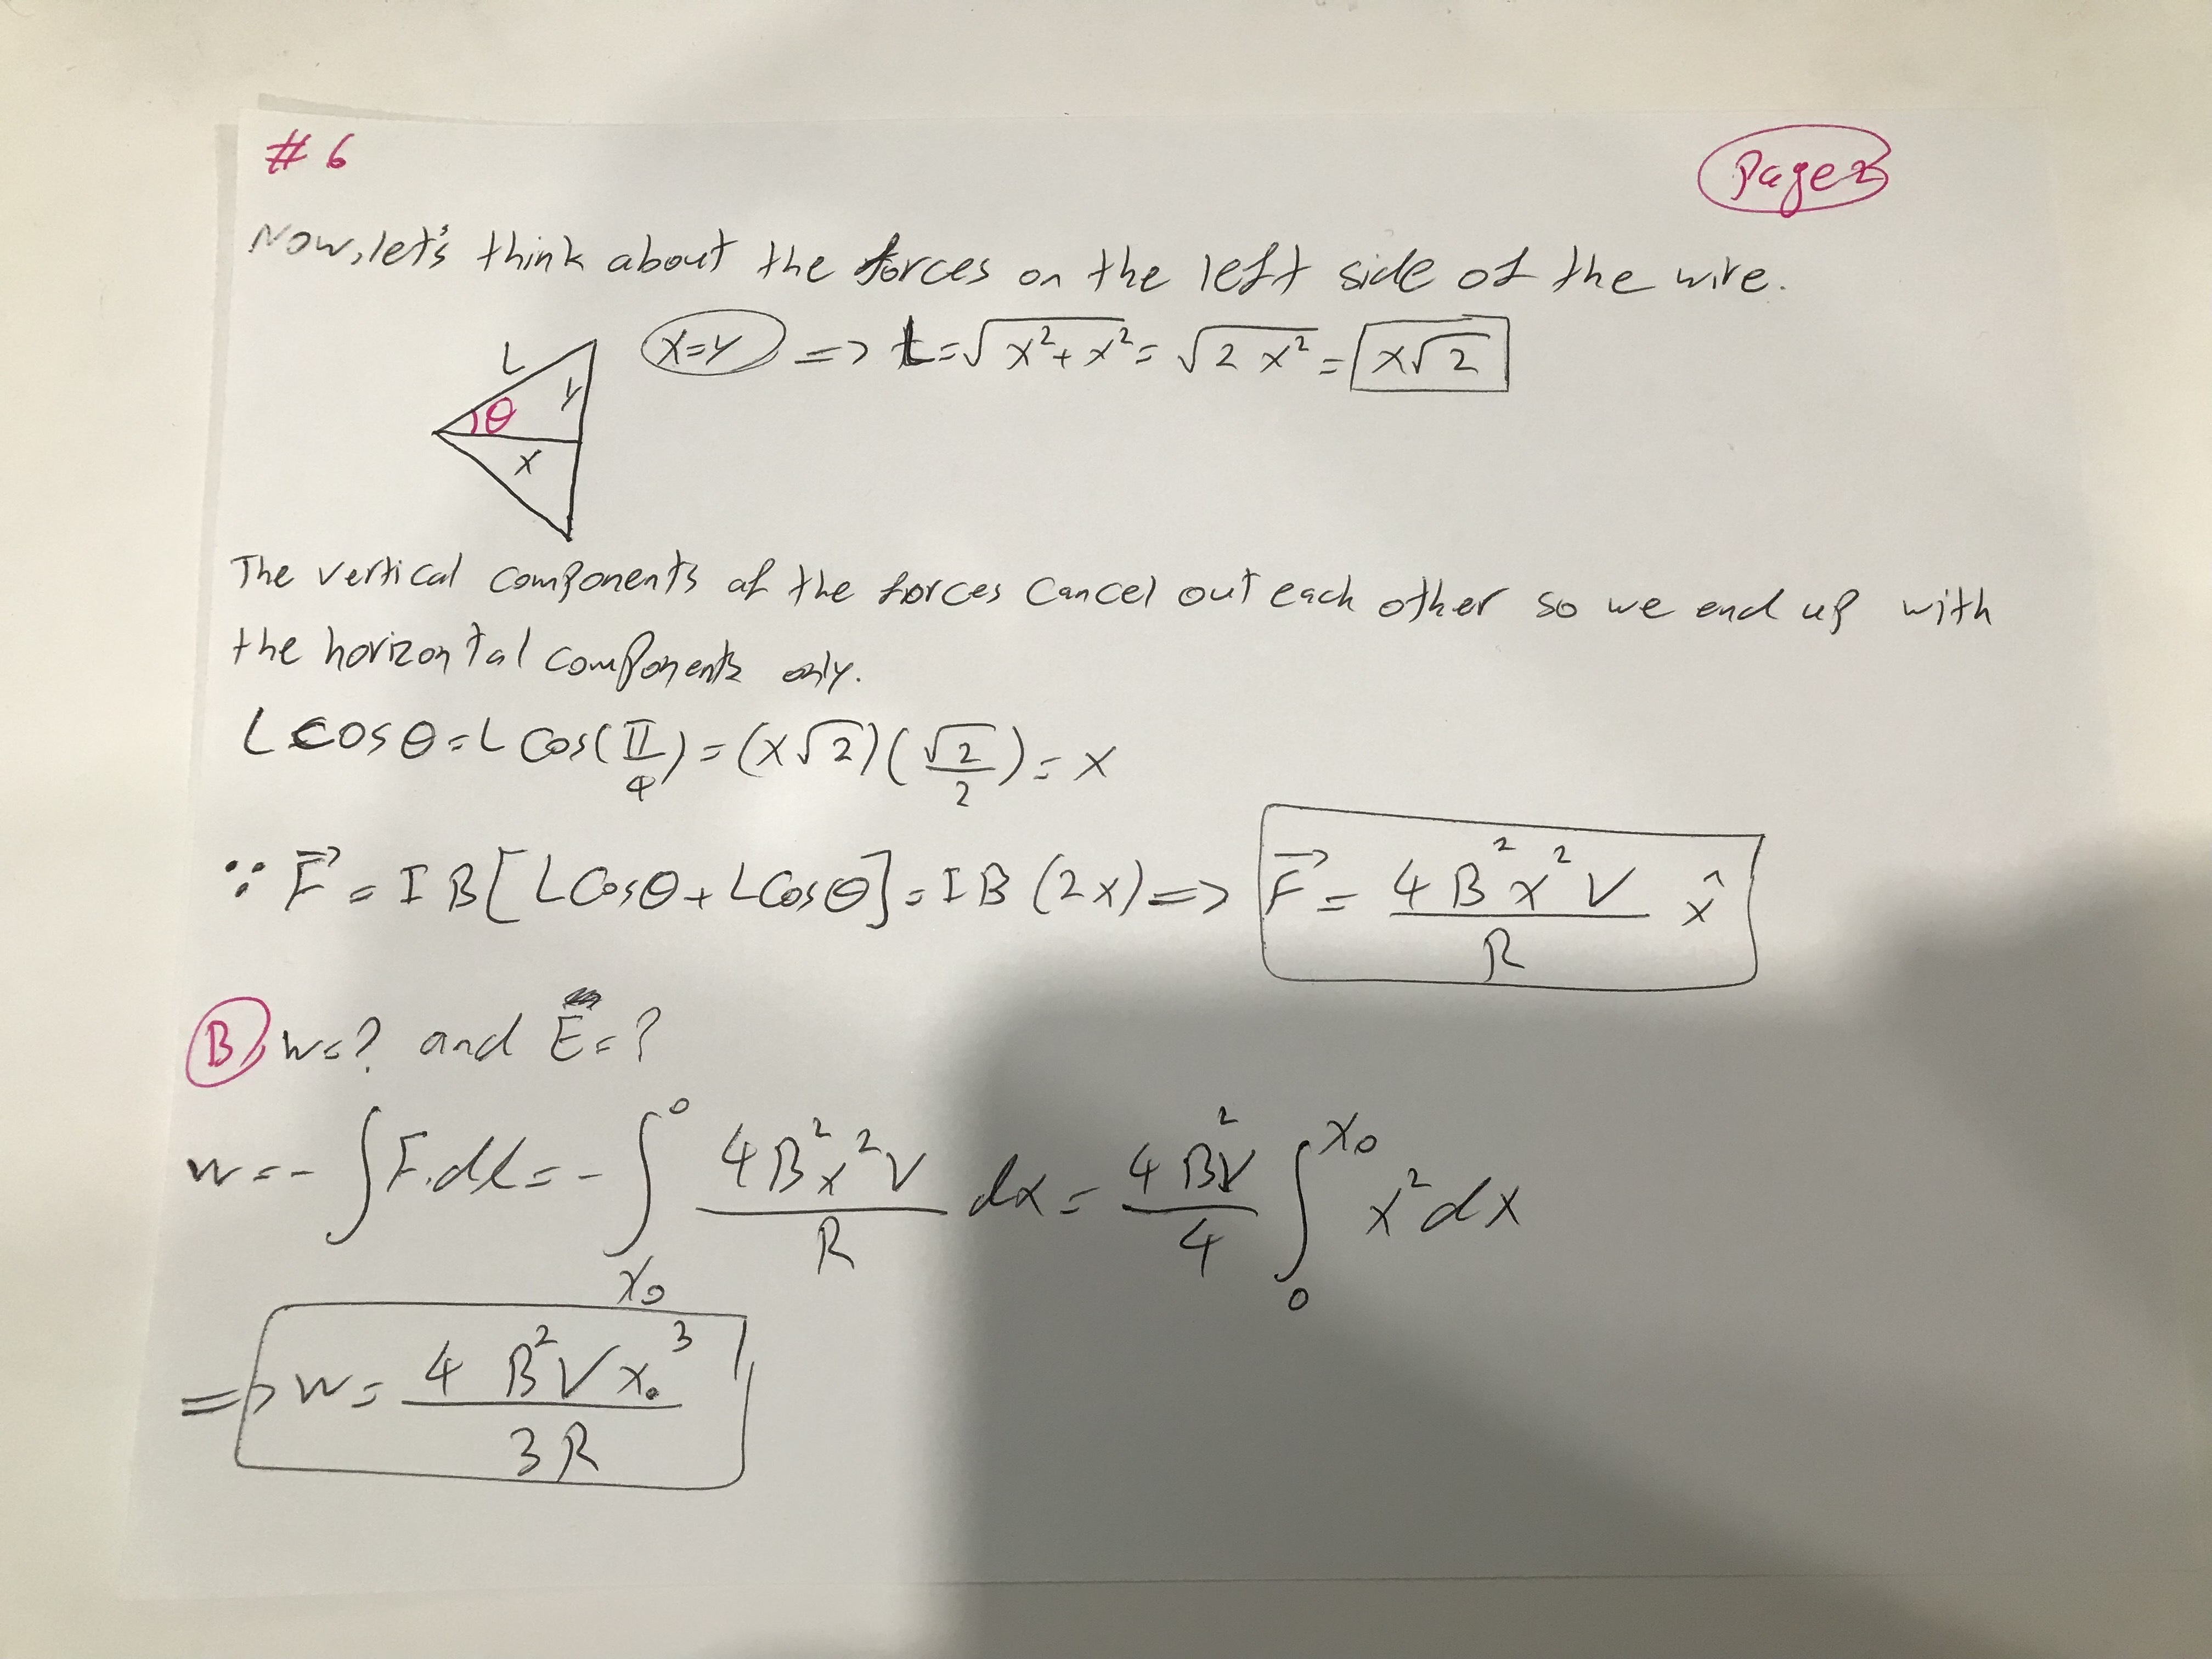
\includegraphics[height=13cm, width=15cm]{6B.jpg}

    \pagebreak

    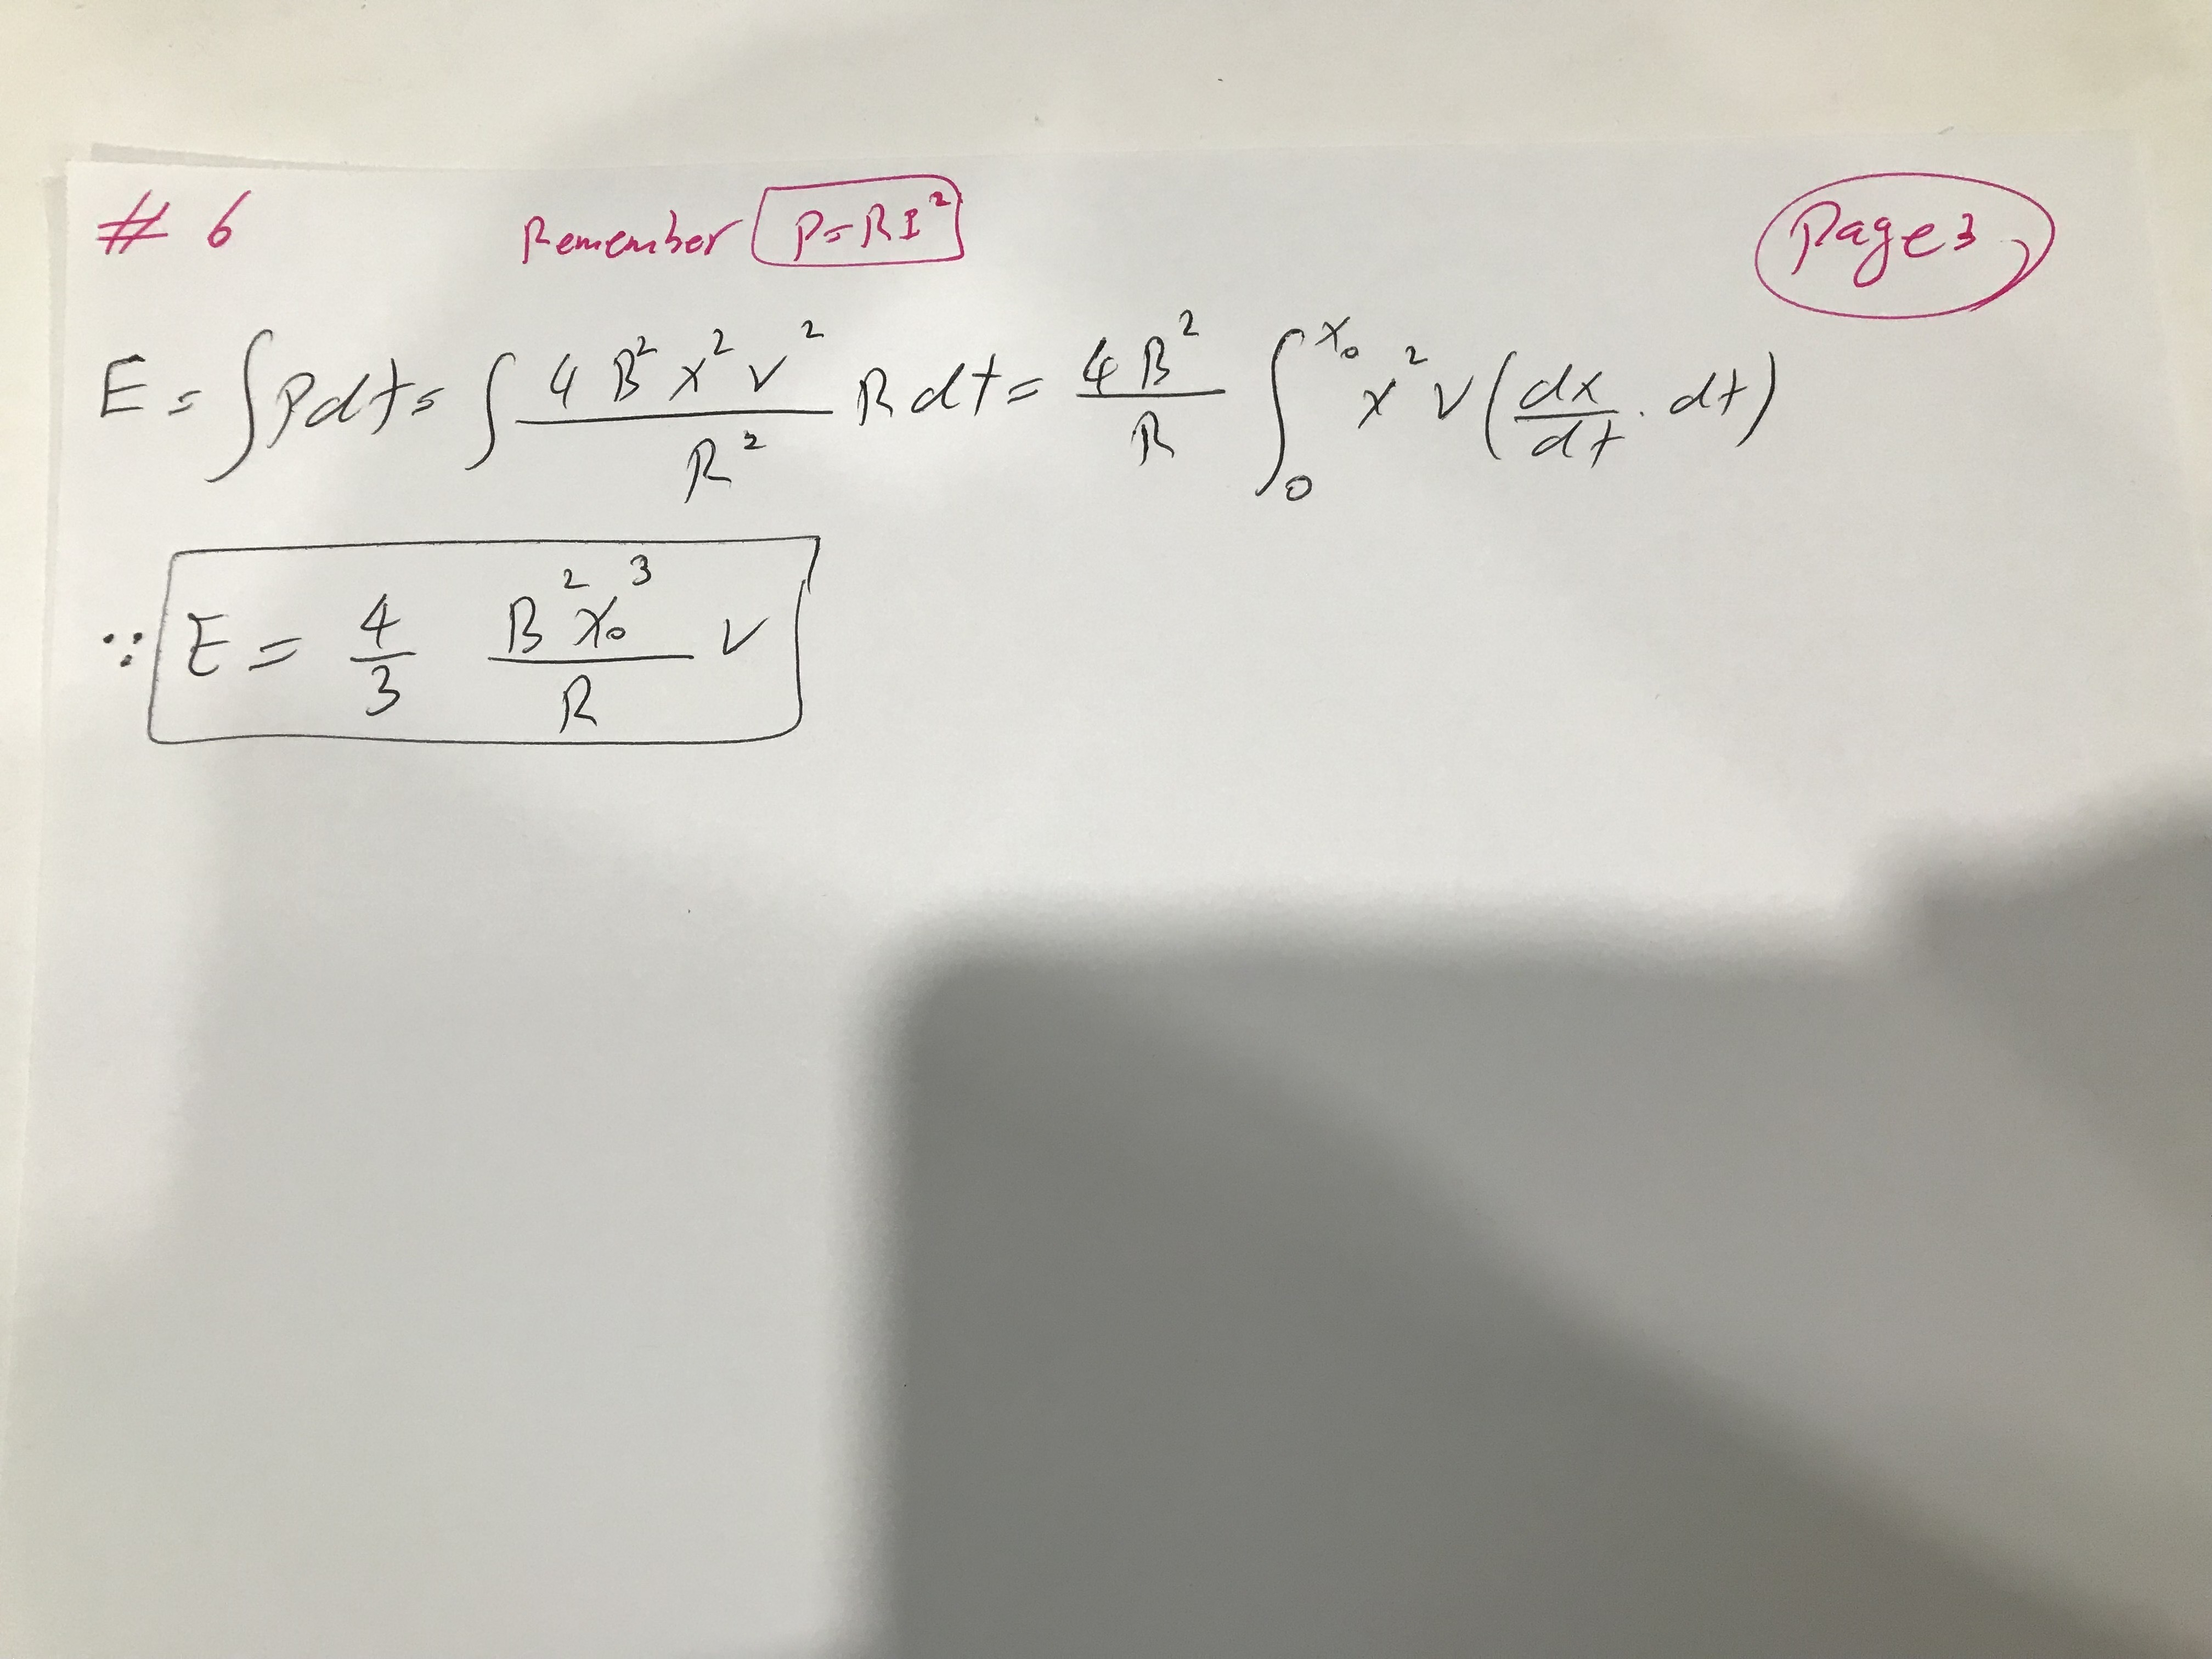
\includegraphics[height=13cm, width=15cm]{6C.jpg}

    \pagebreak

    \item Consider a charged particle of charge $q$ moving at constant speed $v$ along the $\hat{z}$-axis in the 
    $+ \hat{z}$ direction. (Assume that $v<<c$ so you can ignore time dilation, etc.) For a non-relativistic 
    charged particle, the instantaneous electric field is approximately the usual Coulomb field centered about 
    the charge’s instantaneous position. At the moment the charge passes up through the origin, consider a circular loop of
    radius $r$ centered about the $\hat{z}$-axis at some $z>0$. Using Maxwell’s equation (including his correction 
    to Ampère’s law) in integral form, show that the magnetic field $\overrightarrow{B}$ of a moving point charge is 
    $\left(\mu_0 \epsilon_0\right) \overrightarrow{v} \times \overrightarrow{E}$.


    \item A half-infinite wire, $z\leq 0$, carries a current $I$ from negative infinity to the origin, so that a 
    charge, $q(t)$, builds up there. Consider a circle of radius $R$ in the $z=z_0 > 0$ plane, centered (in that plane) about the
    origin of x, y coordinates. Calculate $\bigoint \overrightarrow{B}.\overrightarrow{d\ell}$ around the circle in three
    different ways, by
    \begin{enumerate}
      \item Using the Biot-Savart law.

      \item Using the integrated form of Ampére’s law, as corrected by Maxwell, choosing a surface $S$ that is 
      bounded by the circle but does not intersect the wire.

      \item Using the integrated form of Ampére’s law, as corrected by Maxwell, choosing a surface $S$ that is 
      bounded by the circle and intersects the wire.
    \end{enumerate}


  \end{enumerate}

\end{document}
